% !TeX spellcheck = en_US
\chapter{State of the Art}\label{sota}%

In this chapter, the related works and studies are presented with respect to our research questions and motivation. Additionally,
a wide range of commercial, and non-commercial frameworks/tools have been developed for automotive software integration, configuration, and E/E architecture synthesis. These tools aim to address mapping issues and model software components, including DSE and optimization methods. A comprehensive examination and analysis of these tools are provided in Section~\ref{tools_relatedwork}. Furthermore, we discuss our contributions to the current state of the art.



%\section{Software Architecture Synthesis, Time-triggered Scheduling, and Message Routing }

%There are several approaches, studies, commercial, and non-commercial tools for automotive software integration, configuration, and E/E architecture synthesis focused on mapping problems and modeling of the software components comprising design space exploration(DSE) and optimization methods, which we have comprehensively presented and analyzed in~\cite{askaripoor2022architecture}. In the following, the most related ones are explained.





%Archepotrix is an open-source tool that supports modeling software components, and communication between software components, electronic control units (ECUs), buses, and services. Nevertheless, the tool can optimize the deployment of software components to ECUs based on various objectives, such as redundancy allocation, energy consumption, and cost~\cite{aleti2009archeopterix}. However, It does not support mapping analysis and its solving for multi-core architecture. In addition, the safety-related attributes regarding ISO 26262 are not integrated into this tool except for reliability, and the framework itself supports no model checking and model analysis. Additionally, the covered optimization objectives by ArcheOpterix are restricted, including cost, communication overhead, and data transmission reliability; furthermore, the tool has a limited number of architectural elements. 

%Archepotrix is an open-source tool that assists in modeling software components, communication between components, electronic control units (ECUs), buses, and services. The tool optimizes the deployment of software components to ECUs based on various objectives, such as redundancy allocation, energy consumption, and cost~\cite{aleti2009archeopterix}. However, it does not have the capability to perform mapping analysis and solving for multi-core architecture. Additionally, the tool lacks integration of safety-related attributes as per ISO 26262, with the exception of reliability, and does not provide any model checking or analysis.
%The optimization objectives supported by ArcheOpterix are limited to cost, communication overhead, and data transmission reliability, and the tool has a limited number of architectural elements to choose from.


%MechatronicUML is proposed by Becker et al.~\cite{becker2014mechatronicuml} as an engineering approach to model SW/HW components, specify constraints, and verify the models using model checker UPPAAL for distributed mechatronic systems~\cite{bengtsson1995uppaal}. Nonetheless, this tool has limitations for mapping and software integration in the automotive domain. Firstly, mapping analysis and DSE related to the mapping problem in computing units are not covered by this framework, and MechatronicUML supports no optimization. Furthermore, no safety-related attributes were considered in this tool for modeling, analysis, and solving. In addition, this approach does not focus on multi-core or HPCU modeling and analysis.
%AutoFOCUS3 is another open-source model-based development tool that supports architecture modeling from the requirements to code generation for embedded systems~\cite{aravantinos2015autofocus}. Furthermore, the tool can synthesize hardware platform architectures, including end-to-end latency calculation. It is also able to synthesize and explore optimal deployments and schedules. However, it does not cover the solving approach for the mapping problem considering functional and non-functional requirements to automate mapping configuration and there is no mapping analysis for multi-core platforms. In addition, it supports a limited number of safety attributes (only ASIL level) and optimization goals.
%A model-based approach was introduced in~\cite{hilbrich2011model}, namely Assist,to solve and optimize the deployment of safety-critical applicationson the avionics hardware for distributed systems in the aviation domain. It uses the DSEmechanism to find optimal mapping solutions while considering optimization objectives,including resource usage, weight, and cost. In addition, this Eclipse-based tool can create aperiodic schedule for real-time tasks and ensure a deterministic timing behavior.This framework, however, has some limitations. The specified architectural elementsare extremely limited in terms of hardware and software levels. Moreover, it only supportsredundancy as automotive safety-relevant attributes for mapping problem. Moreover, Assist does not support model checking and model analysis, and the numberof defined optimization goals is limited. 
%OSATE is another open-source tool that implements the architecture analysis and design language (AADL) and supports modeling both aerospace and automotive systems~\cite{feiler2019open, feiler2006architecture}. It supports model checking, schedulability analysis, and flow latency analysis; however, this framework does not use or cover any DSE approaches, e.g., solving mapping problems for multi-core automotive computing units, and, consequently, it supports no optimization. In addition, it covers a limited number of safety attributes.
%An open-source Eclipse platform, called APP4MC, was proposed by~\cite{hottger2017app4mc} which contributes to performance simulation regarding mostly scheduling and timing analysis in multi-core platforms using a model-based development approach while optimizing the solution considering predefined optimization objectives such as load balancing and energy consumption. Nonetheless, this framework does not contribute to automating the deployment of various tasks to various HW elements. APP4MC only analyzes and simulates the task mapping but not solving it. Furthermore, it is restricted in the covered safety attributes and optimization goals, and there are a considerable number of E/E architecture elements which are not considered by AAP4MC.

%To the best of our knowledge, none of the above-mentioned frameworks support communication message routing and time-triggered scheduling for automotive/non-automotive networks. In addition, they introduce not a single-step solving approach for exploring the design space of mapping, routing, and scheduling problems. 

%It should be added that several types of research have investigated message routing and time-triggered scheduling for networks. For instance, Samirnov et al.~\cite{smirnov2017optimizing} present an approach to create message routings and valid schedules in a single-step approach for time-triggered networks. The authors of~\cite{farzaneh2017graphical} present a framework to calculate time-triggered schedules for time-sensitive networking (TSN) networks while fulfilling TSN standards. In~\cite{zhang2014task}, the authors formulate a method to compute time-triggered schedules for tasks over communication links and applications running on network's end stations. 
%However, these works do not support automated mapping and message routing simultaneously while calculating time-triggered schedules for application threads and communication tasks. 

%None of the above-mentioned researches and frameworks provide an approach to synthesize E/E architecture covering mapping and time-triggered scheduling for assigned applications including their threads, single, redundant, homogeneous redundant, and multi-cast message routings creation while calculating time-triggered schedules for communication tasks, supporting path dependency, and applying optimization objectives including end-to-end latency, response time, resource usage, link occupation rate, and cost simultaneously using a single-step solving approach. Furthermore, \textit{E/E designer} offers variously formulated safety-requirements comprising freedom from interference (FFI), redundancy, homogeneous redundancy, and ASIL level. In addition, we evaluate the \textit{E/E Designer} performance by deploying the design-time solutions on an experimental setup which none of above-discussed works have done.

\section{Communication Message Routing and Synthesis of Time-triggered Schedules in Automotive Networks}
  In this section, we go through the most relevant studies to create valid paths over the vehicle network in order to transfer a communication message from a sender to a receiver in the automotive architectures. Moreover, studies and approaches related to the synthesis of time-triggered scheduling are illustrated.
  %Lukasiewycz \emph{et.al}~\cite{lukasiewycz2014system} proposed a graph-based model and a constraint system to create routing of messages generated by an application which is mapped on an ECU in the architecture. The same authors~\cite{lukasiewycz2009combined} introduces a binary encoding strategy for resource allocation, binding the tasks, and routing the messages using Satisfiability (SAT)-encoding for the one-linear objective optimization. 
  \subsection{Communication Message Routing}\label{messagerouting_relatedwork}
  In their work, Lukasiewycz \emph{et.al}~\cite{lukasiewycz2014system} presented a model based on graphs and a constraint system that enables the creation of message routing for applications running on an ECU within an architecture. They also introduced a binary encoding strategy in a previous work~\cite{lukasiewycz2009combined}, which uses Satisfiability (SAT)-encoding to allocate resources, bind tasks, and route messages for optimal one-linear objectives. 
  %An automated approach, for the creation of low-redundant and single routings in automotive architectures while considering predefined optimization goals using SAT-Decoding, was explained in~\cite{smirnov2018automatic}. In this work, mapping of applications on the resources, given to the system as inputs. In addition, the generated routes were optimized based on the number of allocated links and mean-time-to-failure (MTTF) (i.e., defined as the individual failure rate for all architecture components).
  In \cite{smirnov2018automatic}, an automated method was presented for producing automotive architectures that have low redundancy and single routings. The method takes predefined optimization objectives into account by utilizing SAT-Decoding. It involves assigning resources to the system based on the mapping of applications. Generated routes are then optimized based on the number of allocated links and MTTF. MTTF is defined as the individual failure rate for all the components of the architecture. 
  
   This study~\cite{smirnov2017optimizing} focuses on optimizing the communication within automotive networks where multiple systems with varying levels of criticality coexist. 
   The authors propose a message routing and scheduling strategy for time-triggered networks in such environments to ensure efficient and reliable communication. This strategy takes into account the different criticality levels of the messages and assigns appropriate priorities to them to avoid congestion and minimize latency. Optimization is achieved by using mathematical models to determine the best routing and scheduling decisions in real-time. The results of the proposed strategy are evaluated and compared to other existing methods, demonstrating its effectiveness in improving communication performance in automotive mixed-criticality systems.



  
  
  
  %The new Time-Sensitive Networking (TSN) standards improve the safety (e.g. by introducing mechanisms for deterministic timing and high network reliability) of E/E architectures. 
 The recent introduction of TSN standards has further enhanced the safety of E/E architectures, including mechanisms that ensure deterministic timing and high network reliability. 
  IEEE developed TSN standards~\cite{TSN} to address the hard real-time requirements of Ethernet-based distributed applications. The primary goal of these standards is to facilitate the implementation of distributed applications with varying levels of criticality on the same network infrastructure. In particular, the IEEE 802.1DG TSN standard was developed for the automotive industry and includes profiles for secure, highly reliable networks (e.g., utilizing IEEE 802.1CB for seamless redundancy), deterministic latency, and automotive in-vehicle bridged IEEE 802.3 Ethernet networks.
  %Nayak \emph{et.al}~\cite{nayak2016time} present an approach providing real-time guarantees for communication of time-sensitive traffic using transmission scheduling. They utilize integer linear programming (ILP) formulations to calculate schedules. These papers concentrate on the relation between the schedule of the time-triggered traffic and the message routing while, redundant routing is not discussed. 
   Nayak \emph{et.al}~\cite{nayak2016time} propose a method for ensuring real-time communication of time-sensitive data through transmission scheduling. Their approach employs integer linear programming (ILP) formulations to generate schedules. Their work focuses on the relationship between message routing and the schedule of time-triggered traffic, while they do not address redundant routing.
  %The authors in~\cite{gavrilut2017fault} solve an optimization problem for synthesis of TSN-based distributed network topologies and stream routing. This work considers real-time and redundancy requirements of the applications and also defines the cost as an optimization goal to minimize the architecture's cost. An approach is proposed by \cite{smirnov2019variety} for automated routing optimization considering regions within a given network that do not offer any routing variety. Additionally, the authors use an algorithm to find proxy areas in the network. 
   Authors of \cite{gavrilut2017fault} present a solution to an optimization problem that involves the synthesis of TSN-based distributed network topologies and stream routing. This approach considers the applications' real-time and redundancy requirements and aims to minimize the cost of the architecture as an optimization goal. Meanwhile, \cite{smirnov2019variety} introduces an automated approach for optimizing routing that takes the regions in a given network into consideration that lack routing variety. The authors also propose an algorithm for identifying proxy areas in the network.



  
  %However, these studies do not support automated mapping and message routing while calculating time-triggered schedules for application threads and communication tasks. 
    
    %The above approaches create routings for network architectures; however, they consider a predesigned architecture as an input for the constraint system and do not create HR routing. Moreover, none of these studies utilized a model-based development approach.

\subsection{Synthesis of Time-triggered Schedules in Automotive Domain}\label{TT_relatedwork}

There are many studies on time-triggered schedule synthesis. In the following, the most relevant ones in relation to this thesis are discussed. 

Over the past few years, various research studies have been conducted on software integration and architecture synthesis within the automotive domain. One such example is the study conducted by the author in~\cite{terzimehic2018optimization}, who proposed an optimized reconfiguration of industrial automation systems. This study utilized the DSE approach to determine optimal architectural configurations for control applications by taking into account constraints and optimization goals.
%Similarly, a framework was presented in \cite{zheng2016next} to provide architecture modeling for automotive systems. The authors claimed that their framework facilitates system integration while utilizing optimization approaches. In addition, it considers validation for different design metrics including reliability, and timing. 
Similarly, a framework was introduced in \cite{zheng2016next} that offers a model for architecture in automotive systems. Authors claimed that the framework they presented enables integration of systems while incorporating optimization techniques and also takes into account validation for various design metrics, such as reliability and timing~\cite{askaripoor2022architecture}.
%The research paper \cite{zheng2005extensible} presents an approach to reduce development and re-verification efforts in the automotive domain using time-triggered scheduling scheme. A method is introduced by authors in \cite{smirnov2017optimizing} to create valid time-triggered schedules for communication frames routing over network's links exploiting 0-1 ILP formulation.
In \cite{zheng2005extensible}, the authors discuss a time-triggered scheduling scheme that can help to reduce development and re-verification efforts in the automotive domain. Meanwhile, \cite{smirnov2017optimizing} presents a methodology for generating valid time-triggered schedules for routing communication frames over network links. This approach leverages a 0-1 ILP formulation.
%Authors of \cite{sagstetter2015multischedule} introduce a method for time-triggered schedule synthesis of automotive hardware architectures creating release times of periodic tasks and messages. Moreover, the proposed approach supports multi-schedule synthesis for different variants of hardware architecture. Additionally, the authors run several tests to evaluate the performance of their approach including resource utilization, run-time evaluation for variant and non-variant use cases, and end-to-end delay analysis. 
In \cite{sagstetter2015multischedule}, the authors describe a technique for synthesizing time-triggered schedules for automotive hardware architectures. This method generates release times for periodic tasks and messages and can also support multi-schedule synthesis for different hardware architecture variants. Authors also conduct several evaluations to measure the effectiveness of their approach, including tests for resource utilization, run-time evaluation for both variant and non-variant use cases, and end-to-end delay analysis.


This study \cite{lukasiewycz2012concurrent} proposes a methodology to optimize time-triggered automotive systems with a particular focus on FlexRay bus scheduling. An extended architecture model of this work considers resource utilization and configuration, path delays. Furthermore, the authors present a strategy to enable an efficient selection of architecture decisions to avoid an infeasible schedule. Authors of~\cite{farzaneh2017graphical} propose a graphical modeling tool to reduce configuration effort and overhead by automating gate control list (GCL) schedule synthesis for TSN networks. Moreover, they use a model-based development approach to develop their framework and apply logic programming to transform a designed graphical network to a network knowledge base. Zhang et al.~\cite{zhang2014task} formulate a method for computing time-triggered schedules for tasks routing over communication links and applications running on network end stations. Authors in \cite{8889667} aim to address the problem of computing no-wait schedules and multi-path routings for large-scale TSN networks. This study introduces an iterated ILP-based scheduling approach to achieve high scheduling scalability and also provides a degree of conflict (DOC)-aware multi-path routing methodology to achieve fault tolerance. Developing proper scheduling approaches, as well as modeling and verification tools, including experimental setups, is essential in traffic planning and verification of TSN networks. However, this process can be time-consuming and requires advanced expertise, which highlights the need for motivation in this area of research~\cite{craciunas2016scheduling, ashjaei2017schedulability, farzaneh2017time}.


\section{Software Architecture Synthesis-related Studies}\label{SW_synthesis_relatedwork}

This section presents related papers on software architecture and E/E system synthesis, including those that consider safety requirements.

\subsection{Software Architecture Synthesis}

In \cite{zimmermann2018optimization}, a new methodology is presented for solving optimization problems in engineering design, particularly those with a nested structure of design parameters. The authors introduce the concept of "existence-dependent parameters," which are found to arise in various problems, including the optimization of system architectures. 
%This paper advocates for a model-driven approach to solving these problems and presents a prototype tool that integrates various domain-specific tools. The methodology and tool are demonstrated using an example from the design of distributed embedded systems, involving hardware architecture and software mapping.
A model-driven approach is proposed in this study to address these issues. A prototype tool is introduced that integrates multiple domain-specific tools. A methodology and tool are demonstrated in the context of a distributed embedded system design example, which includes hardware architecture and software mapping.
%This work \cite{7336300} describes a new approach to analyzing the timing of embedded computer systems. The authors note that current methods for analyzing timing in these systems are limited because they do not take into account the distributed, layered, and heterogeneous nature of these systems. 
An analysis of timing in embedded computer systems is the focus of this study \cite{7336300}, which proposes a new approach. Authors observe that current methods are inadequate as they do not consider the layered, distributed, and heterogeneous nature of these systems.
%The proposed framework is designed to be more flexible and versatile, allowing developers to select and apply a set of timing analysis tools that are best suited for each individual subsystem. The framework takes into account the dependencies between subsystems to produce a comprehensive, end-to-end timing analysis.
The framework proposed is aimed to be more adaptable and multipurpose, giving developers the liberty to choose and utilize a collection of timing analysis tools that would be appropriate for each individual subsystem. This tool considers the interdependence among the subsystems and delivers a thorough timing analysis from end-to-end.
%The paper\cite{8560591} describes a methodology for finding optimal deployment configurations for systems based on the IEC 61499 standard. The approach involves exploring different design options, or the "design space", to determine the best configuration for the specific requirements and constraints of the system. 
A methodology presented in \cite{8560591} outlines a process for identifying the best deployment configurations for systems that adhere to the IEC 61499 standard. This approach involves exploring various design options within the system's design space to identify the optimal configuration that satisfies the given requirements and constraints.
%The goal is to improve the performance and efficiency of the system through proper deployment. The results of the design space exploration are used to calculate the deployment configurations that meet the desired specifications.
The objective is to enhance the system's efficiency and performance by deploying it in an appropriate manner. DSE outcomes are utilized to compute deployment configurations that fulfill the desired specifications.


 


\subsection{E/E System Synthesis Considering Safety Requirements}

%Mody~\cite{mody2018understanding} presents an explanation regarding AD/ADAS topologies by analyzing two system topologies as two examples. Besides, the authors have compared these two topologies by considering several parameters including bandwidth, functional safety, number of ECU, cost, etc. 
Mody~\cite{mody2018understanding} provides an analysis of two automated driving (AD)/ADAS system topologies to explain their characteristics. The study compares the two topologies based on various parameters, such as bandwidth, functional safety, number of ECUs, and cost.
%Also, system partitioning with focus on the AD/ADAS domain corresponding to each topology was explained in this work.
This work also explains the system partitioning specific to the AD/ADAS domain for each topology.
%Zerfowski et al.\cite{zerfowski2019functional} discuss upcoming E/E architectures within the automotive domain as well as related aspects to the E/E architecture components comprising cyber security, energy management, appropriate middleware, etc.% Also, the relevant challenges to these aspects are addressed in this study. 
The authors of \cite{zerfowski2019functional} examine the future E/E architectures in the automotive industry and the components that will be necessary for these architectures, such as cyber security, energy management, and appropriate middleware.
%The network used within the automotive domain, specifically the Ethernet network, has been analyzed in terms of safety aspects by this paper \cite{van2018functional}. Also, a bit flip comparison between CAN based and Ethernet-based networks has been done.
\cite{van2018functional} examines the safety aspects of the Ethernet network used in the automotive domain, and provides a comparison of bit flip between Ethernet-based and CAN-based networks.
Furthermore, this study presents a short overview of future automotive networks considering some functional safety characteristics such as seamless redundancy.
%Asim et al.\cite{abdulkhaleq2017using} propose a safety approach to improve the safety of the architecture utilized in an autonomous car and assess the architectural design of the self-driving system at the development process.  
Authors of \cite{abdulkhaleq2017using} suggest a safety method to enhance the safety of the architecture employed in an autonomous vehicle, as well as evaluate the architectural design of the self-driving system during the development stage. In addition, the introduced approach functions as a hazard analysis technique, named system theoretic process analysis (STPA), in compliance with ISO 26262.


%A method is declared for safety-critical applications within the automotive domain which is appropriate for a centralized ECU by Yoneda et al.\cite{yoneda2019network}. It is a NOC (Network-on-Chip) platform and is designed to mitigate link faults as well as handle delay faults. 
Yoneda et al.~\cite{yoneda2019network} propose a technique for safety-critical applications in the automotive industry that is suitable for a centralized ECU. This technique utilizes a network-on-chip (NOC) platform specifically designed to address link and delay faults.
%Adina et al.\cite{aniculaesei2016towards} has proposed an approach for safety verification of autonomous systems that the static verification technique, at design time, is combined with dynamic one, at run time, to transfer the results of static verification to run time environment. Additionally, the authors presented a real-time monitoring method to diagnose the correctness of the system assumptions at run time based on the suppositions made at design time.
In this work, Aniculaesei and colleagues~\cite{aniculaesei2016towards} put forward a method for ensuring the safety of autonomous systems. This method involves combining static verification techniques during the design phase with dynamic verification techniques during operation, allowing for the transfer of results from the design phase to the run time environment. Furthermore, the authors proposed a real-time monitoring approach to assess the accuracy of the system assumptions during operation based on the assumptions made during the design phase.
%This study \cite{chitnis2017enabling} points out to safety requirements at the software level of a self-driving car consisting of listed methods 1. Redundancy at different levels of system 2. Software and hardware architecture proposal based on redundancy requirements 3. Usage of freedom from interference (FFI) technique 4. Run time monitoring of the software and hardware due to detect and avoid run-time failures. 
 In this study \cite{chitnis2017enabling}, the focus is on identifying safety requirements for the software of a self-driving car. The study lists four methods that can be used to ensure safety:
\begin{itemize}
    \item Implementing redundancy at multiple levels of the system.
    \item Designing the software and hardware architecture based on redundancy requirements.
    \item Utilizing FFI technique.
    \item Monitoring the software and hardware at runtime to detect and avoid any potential failures.

\end{itemize}

 %The reliability of a heterogeneous automotive system using Automotive Safety Integrity Level (ASIL) decomposition has been studied by the authors in~\cite{xie2017minimizing}. They presented two heuristic algorithms to improve the reliability goal while minimizing the development cost for each ASIL decomposition scheme. This work calculates the reliability based on tasks mapped on the ECUs and their failure rates. 
 In \cite{xie2017minimizing}, the authors investigate the reliability of a heterogeneous automotive system using ASIL decomposition. They propose two heuristic algorithms to increase reliability while minimizing development costs for each ASIL decomposition scheme. The approach calculates reliability by considering tasks mapped on the ECUs and their corresponding failure rates.
%The authors of~\cite{gan2014tradeoff} and~\cite{tamacs2011optimization} have focused on meeting the real-time requirement of distributed automotive applications while optimizing the development cost.
In both \cite{gan2014tradeoff} and \cite{tamacs2011optimization}, the authors aim to address the real-time requirements of distributed automotive applications while optimizing development costs.
%0The paper~\cite{zimmermann2018optimization} proposes a new methodology for solving optimization problems in engineering design, with a focus on problems where the design parameters form a nested structure. The concept of "existence-dependent parameters" is introduced and shown to appear in problems such as optimizing system architectures.
 %A safety monitoring method at run time in an autonomous system is introduced by Haupt\cite{haupt2019runtime}. This method utilizes a set of safety rules to detect safety-critical violations in the system. It also provides self-consciousness ability to keep the system safe operational at run time.
 Haupt introduced a safety monitoring method for autonomous systems in 2019, as documented in \cite{haupt2019runtime}. This method uses a collection of safety rules to identify any safety-critical violations that may occur in the system during runtime. Additionally, the method provides the system with the ability to maintain self-awareness and ensure safe operations while in use.
\begin{comment}
\begin{figure}[t]
\centering
\includegraphics[width=\textwidth]{Approach_ETFA.pdf}
\caption{The approach procedures including three steps.}
\label{fig6}
\end{figure} 
\end{comment}
 %Mulkul et al.\cite{gosavi2018application} propose three models at the architectural level for driverless cars which assure functional safety of E/E components based on ISO26262. A model-based method to analyze the safety of an automated driving system is addressed by this group of researchers \cite{tlig2018autonomous}. 
 In their work, Gosavi et al. \cite{gosavi2018application} put forward three different architectural models for autonomous vehicles that ensure the functional safety of their E/E components in accordance with ISO26262~\cite{iso26262}. Another group of researchers, Tlig et al. \cite{tlig2018autonomous}, focus on a model-based approach for assessing the safety of automated driving systems.
 %In this approach environment as well as perception, fusion, and control units used in an autonomous car have been modeled. After applying a further step, named sequence extraction and analysis, to verify a specific scenario, this model is simulated which visualizing a car and its surrounded environment.\newline
 In this approach, a model can be developed that includes the environment, perception, fusion, and control units for an autonomous car. This methodology also involves sequence extraction and analysis to validate particular scenarios. The model is then simulated, which includes visualizing the car and its surroundings.
% \subsection{morteza stuff}
% Networking in the E/E architecture plays an essential role in ensuring safety guarantees. In particular, the successful development of the L4 and L5 stages of autonomous driving requires strict timing, high availability, and reliability of the communication system. The importance of these prerequisites becomes clearer in the scenarios without a driver as a fallback (no steering wheel in the car). In these situations, the safety requirements for the network as a part of the E/E architecture will reach the ASIL-D level which has not been the case so far. Therefore the consideration of safety aspects in the design phase of the architecture from the beginning is of significant importance to support fail-operation application development. 
 %Time-Sensitive Networking (TSN) standards~\cite{TSN} developed by the Institute of Electrical and Electronics Engineers (IEEE) address the hard real-time requirements of Ethernet-based distributed applications. The main objective of these standards is to support the implementation of distributed applications with different levels of criticality in the same network infrastructure. Especially for the automotive domain developed IEEE 802.1DG TSN standard~\cite{b41}, specifies profiles for secure, highly reliable (e.g. using IEEE 802.1CB for seamless redundancy~\cite{b50}), deterministic latency, automotive in-vehicle bridged IEEE 802.3 Ethernet networks. T
 %Traffic planning and verification of TSN networks require advanced expertise and are time-consuming; a motivation to develop adequate scheduling approaches~\cite{craciunas2016scheduling}, modeling and verification tools (including experimental setups)~\cite{ashjaei2017schedulability, farzaneh2017time}. 
 
 %Developing proper scheduling approaches, as well as modeling and verification tools, including experimental setups, is essential in traffic planning and verification of TSN networks. However, this process can be time-consuming and requires advanced expertise, which highlights the need for motivation in this area of research~\cite{craciunas2016scheduling, ashjaei2017schedulability, farzaneh2017time}.
 
 %Moreover, recent works also deal with consideration of safety aspects in routing decisions~\cite{b39,b40} to increase the reliability of the critical applications. 
%\todo[inline]{A key problem with much of the literature on safety aspects of the autonomous vehicles specifically their architecture and topology is that there is no approach to generate the architecture based on predefined rules in compliance with automotive standards used in the self-driving cars to the best of our knowledge.***********}
%The mentioned solutions assume a predefined topology and analyze the fulfillment of the safety requirements (e.g. timing and routing). However, they do not address requirement-based generation of the topology. 









\section{Task Mapping in Multi-Core Computing Units}\label{multicore_relatedwork}
%As discussed before, in this section the current mapping approaches and methods and studied optimization objectives for task mapping in multi-core platforms are illustrated. 

As previously discussed, this section will outline the current mapping techniques and methods, as well as the optimization objectives for task mapping in multi-core platforms.






\subsection{Mapping Techniques}
%Static or design-time mapping utilizes all system information (e.g., hardware and application properties) to find the optimal solution. In addition, this type of mapping is appropriate when there is a set of predefined requirements for the applications as well as the hardware. In other words, the mapping problem, including changing application/hardware requirements, cannot be solved dynamically with design-time methodology. Solutions with higher quality can be acquired in the design-time mapping problem rather than the run-time mapping problem due to less limitation of the computational power.

Static or design-time mapping uses all available system information, including hardware and application properties, to find the optimal solution. This type of mapping is most suitable when there are predefined requirements for both the applications and hardware, as it cannot dynamically address changes in application or hardware requirements. Subsequently, it cannot dynamically be solved using design-time methodology. As a result, solutions of higher quality can be achieved through design-time mapping due to the lack of limitations in computational power compared to run-time mapping~\cite{askaripoor2022architecture}.





%\textbf{Design-Time Mapping}: There are several design-time mapping algorithms such as graph-theoretic algorithms, mathematical programming algorithms, and heuristic-based algorithms. In graph-theoretic algorithms, the application is partitioned into separate tasks (can be allocated to the cores for execution) to use the fundamental parallelism~\cite{gupta2021mapping},~\cite{deveci2015hypergraph}. This approach includes various theory methods including Levelized Weight Timing \cite{shivle2004static}, Shortest tree~\cite{bokhari1981shortest}, Max-Min~\cite{braun2001comparison}, hyper-graph~\cite{deveci2015hypergraph}, A$^{*}$~\cite{shivle2004static}, and Kahn Process networks~\cite{castrillon2012communication}. 

\subsubsection{Design-Time Mapping} There are a number of algorithms used for design-time mapping, including graph-theoretic algorithms, mathematical programming algorithms, and heuristic-based algorithms. In graph-theoretic algorithms, the application is divided into separate tasks, which can then be assigned to the cores for execution and take advantage of parallelism~\cite{gupta2021mapping},\cite{deveci2015hypergraph}. This approach encompasses various theories such as Levelized Weight Timing \cite{shivle2004static}, Shortest tree~\cite{bokhari1981shortest}, Max-Min~\cite{braun2001comparison}, hyper-graph~\cite{deveci2015hypergraph}, A$^{*}$~\cite{shivle2004static}, and Kahn Process networks~\cite{castrillon2012communication}.





%Another design-time approach to solve the mapping problem is mathematical programming, where the requirements are transformed into mathematical inequalities. After that, by utilizing different mathematical programming solutions including mixed integer linear programming (MILP)~\cite{niemann1997algorithm}, Branch \& Brand~\cite{hu2005energy}, constraint programming (CP)~\cite{bhatti2012memory}, and integer linear programming (ILP)~\cite{kaida2012task}, the inequalities are solved. In the mathematical programming approach, the optimal solution is always guaranteed as long as the complexity of the mapping problem does not become NP. In the case of the NP problem, heuristic-based algorithms can be used. 

Another design-oriented method for resolving the mapping problem is through mathematical programming, where the requirements are translated into mathematical inequalities. These inequalities are then solved through various mathematical programming solutions, including mixed-integer linear programming (MILP)~\cite{niemann1997algorithm}, Branch \& Bound~\cite{hu2005energy}, constraint programming (CP)~\cite{bhatti2012memory}, and ILP~\cite{kaida2012task}. This approach provides an optimal solution as long as the mapping problem does not fall into the category of NP problems. In such cases, heuristic-based algorithms can be employed.






%The last design-time approach is heuristic-based algorithms. As mentioned before, with increasing the problem complexity and proximity to an NP problem (e.g., increasing the number of cores and complexity of the application requirements), finding the optimal solution is infeasible in the desired time by utilizing mathematical programming algorithms. Therefore, heuristic algorithms are presented to discover a solution which may not be the best of all the solutions to this problem or may approximate the exact solution in a more faster and efficient fashion.
The final design-time approach is the utilization of heuristic-based algorithms. As previously stated, as the complexity of the problem and proximity to an NP problem increases (for example, with an increase in the number of cores and the complexity of application requirements), finding an optimal solution through mathematical programming algorithms becomes unfeasible within the desired time frame. Hence, heuristic algorithms are introduced to provide a solution that may not necessarily be the best, but can still approximate the exact solution in a faster and more efficient manner.






%They classify alternatives in search algorithms at each branching step based on current information to decide which branch to go after. Heuristic algorithms can be divided into Population-Based and Single Solutions. For example, the greedy randomized adaptive search procedure (GRASP) \cite{pascual2011optimization}, simulated annealing (SA)~\cite{giannopoulou2014mapping}, and Tabu search~\cite{braun2001comparison}, which utilize iterative search methods, are considered as the Single solution algorithms. Also, there are several other heuristic-based algorithms which are categorized as Population-based including genetic algorithm (GA)~\cite{gan2016minimizing}, ant colony optimization (ACO)~\cite{ferrandi2010ant}, and particle swarm optimization (PSO)~\cite{xu2016set}.  

The alternative options in search algorithms are classified at each branching step based on the available information in order to determine the next branch to follow. These heuristic algorithms can be further divided into two categories: Population-Based and Single Solutions. for example, single solution algorithms refer to iterative search methods, such as greedy randomized adaptive search procedure (GRASP) \cite{pascual2011optimization}, simulated annealing (SA)\cite{giannopoulou2014mapping}, and Tabu search\cite{braun2001comparison}. These algorithms are known for utilizing an iterative search process. In addition to these algorithms, there are several other heuristic-based algorithms that fall under the category of population-based, such as genetic algorithms (GA)\cite{gan2016minimizing}, ant colony optimization (ACO)\cite{ferrandi2010ant}, and particle swarm optimization (PSO)~\cite{xu2016set}.





\subsubsection{Run-Time Mapping} %In this type of mapping, the tasks assignments to various cores are performed when the applications are executing. The required time to find a feasible and optimal solution plays a critical role in this mapping methodology. %According to~\cite{singh2013mapping, gupta2021mapping}, run-time mapping can be divided into two approaches: On-the-fly mapping and Hybrid mapping. When task allocation is completely done online or during application execution (i.e., without using offline or design-time knowledge) this is interpreted as On-the-fly mapping. While in Hybrid mapping, the task planner uses the offline/design-time mapping result to perform task assignments dynamically. This approach takes advantage of both run-time and design-time techniques. Similar to design-time, there are three well-known algorithms which can be utilized for run-time mapping such as Greedy~\cite{carvalho2007heuristics}, Feedback control theoretic, and Heuristic-based algorithms~\cite{gupta2021mapping}.
In this type of mapping, the allocation of tasks to various cores is carried out during the execution of applications. The amount of time required to find a feasible and optimal solution is a crucial factor in this mapping approach. Run-time mapping can be categorized into two approaches, On-the-fly mapping and Hybrid mapping, as reported in~\cite{singh2013mapping, gupta2021mapping}. On-the-fly mapping refers to a scenario where task allocation is performed online or during application execution without utilizing any offline or design-time information. While in Hybrid mapping, the task planner leverages the results of offline or design-time mapping to perform dynamic task assignments. This approach combines the benefits of both run-time and design-time techniques.
For run-time mapping, there are three commonly used algorithms that can be utilized, including Greedy~\cite{carvalho2007heuristics}, Feedback control theoretic, and Heuristic-based algorithms~\cite{gupta2021mapping}. These algorithms offer a range of options for run-time mapping tasks.



\subsection{Optimization Parameters in Mapping}\label{optimization}
%To improve the quality of task assignment in multi-core processors, either in static or dynamic mapping, some key requirements must be considered.
For the purpose of enhancing the task assignment quality in multi-core processors, whether through static or dynamic mapping, it is crucial to take into account certain critical requirements.





\subsubsection{Performance}%The design of multi-core processors has been becoming more and more complex with the increasing number of applications as well as their requirements. Various design-time and run-time approaches have been developed to optimize the performance of mapping (i.e., reducing task execution time during task allocation~\cite{kaida2012task} or increasing CPU utilization). The performance of a multi-core system can be assessed by measuring execution time, latency, response time, and throughput as the evaluation metrics~\cite{mehrara2009multicore}. 
The design of multi-core processors has grown increasingly complex due to the growing number of applications and the increasing requirements placed on them. To optimize performance and improve mapping, various design-time and run-time approaches have been developed, such as reducing task execution time during task allocation~\cite{kaida2012task} or increasing the utilization of the central processing unit (CPU).
When evaluating the performance of a multi-core system, several metrics can be used, including execution time, latency, response time, and throughput~\cite{mehrara2009multicore}. These metrics allow for an assessment of the system's efficiency and effectiveness in executing tasks.




\subsubsection{Power Consumption} %As electric vehicles are becoming more popular and most of autonomous cars will be electric-based, saving electric power has a significant impact on providing an optimized E/E system for the vehicle. As a result, reducing energy consumption during application mapping in multi-core computational units plays a pivotal role in mapping optimization~\cite{xie2018reliability}. Based on~\cite{peressmulti}, minimizing cache miss results in energy reduction of a system by 76 percent. 
Given the increasing popularity of electric vehicles, particularly in the realm of autonomous cars, energy conservation plays a critical role in optimizing the E/E system of the vehicle. Minimizing energy consumption during the application mapping process in multi-core computational units is a critical factor in optimizing the mapping process~\cite{xie2018reliability}. Research has shown that reducing cache miss rates can lead to a substantial decrease in energy consumption, with a 76 percent reduction in energy usage being reported in~\cite{peressmulti}.





\subsubsection{Reliability} %Another important parameter that must be considered as an optimization goal in multi-core computing units is reliability. ISO 26262 has introduced different ASILs to ensure the reliability of the system~\cite{iso26262}. System reliability can be evaluated using the mean time to failure (MTTF), mean time between failures (MTBF), and mean time to repair (MTTR) as failure metrics~\cite{das2014communication}. For example, system reliability is improved in~\cite{huang2009lifetime} utilizing the SA approach. This paper calculates the MTTF by using the temperature variation of cores. Based on this definition, task allocation to the cores is performed in such a way that MTTF is minimized.
When optimizing multi-core computing units, it is essential to take into account reliability as a key factor. ISO 26262 has established various ASILs to guarantee the reliability of the system~\cite{iso26262}. The reliability of the system can be evaluated through the use of MTTF, MTBF, and MTTR as failure metrics~\cite{das2014communication}. As an illustration of the benefits of the SA approach, improved system reliability is demonstrated in~\cite{huang2009lifetime}. The study calculates the MTTF by considering the temperature variations of the cores. Based on this calculation, task allocation is performed in a manner that minimizes the MTTF.





%There are several works regarding the static mapping problem comprising various optimization objectives that have utilized the ILP method. For instance,~\cite{kaida2012task,niemann1997algorithm,ding2013shared,coskun2008temperature} have studied the design-time mapping problem in homogeneous multi-core architecture using the ILP method while optimizing their solutions considering performance, energy consumption, and temperature as the optimization parameters. Authors in~\cite{girault2019erpot} utilized the same method to solve mapping for a heterogeneous architecture, including different optimization goals such as execution time, reliability, and temperature. Furthermore,~\cite{giannopoulou2014mapping,hartman2010case,huang2009lifetime,das2014combined} studied the mapping problem of homogeneous architecture in design-time using heuristic-based approaches including SA, ACO, and GA while optimizing the final solution based on response time, reliability, and energy consumption. 
A considerable number of studies have been conducted on the topic of the static mapping problem, and many of these have used the ILP method. For example, \cite{kaida2012task,niemann1997algorithm,ding2013shared,coskun2008temperature} focuses on the design-time mapping problem in a homogeneous multi-core architecture and utilized the ILP method to optimize their solutions. These studies aimed to optimize parameters such as performance, energy consumption, and temperature.
In~\cite{girault2019erpot}, the authors employed a similar approach to address the mapping issue in a heterogeneous architecture, considering various optimization objectives such as execution time, reliability, and temperature. Other studies, including~\cite{giannopoulou2014mapping,hartman2010case,huang2009lifetime,das2014combined}, have explored the mapping problem for homogeneous architecture during the design phase by employing heuristic-based methods, such as SA, ant ACO, and GA, to optimize the final solution based on factors such as response time, reliability, and energy consumption.

%Several pieces of research have been done to assign tasks to multi-core processors dynamically.~\cite{kinsy2014algorithms,lee2014workload,liu2013dynamic} worked on the heterogeneous architecture to perform run-time mapping using the ILP method. They also optimized their solution, considering performance and power consumption as the optimization goals. While~\cite{bolchini2016combined} utilized the heuristic method (i.e., Age Balancer Heuristics) to execute dynamic mapping on heterogeneous architecture while aiming to minimize computation energy and improve reliability.
A significant amount of research has been conducted to dynamically allocate tasks to multi-core processors. For example, studies by Kinsy et al.~\cite{kinsy2014algorithms}, Lee et al.~\cite{lee2014workload}, and Liu et al.~\cite{liu2013dynamic} focused on heterogeneous architectures and employed the ILP method to perform the run-time mapping. These studies aimed to optimize their solutions with respect to performance and power consumption. On the other hand, Bolchini et al.~\cite{bolchini2016combined} utilized a heuristic approach, specifically the Age Balancer Heuristics, for dynamic mapping on heterogeneous architectures with the aim of minimizing computation energy and enhancing reliability.
%Therefore, with an increase in demand for higher efficiency of mapping in terms of the aforementioned optimization parameters, new challenges have appeared in multi-core processors. These challenges can include thermal management in integrated circuits (ICs), machine learning approaches to perform efficient mapping, and quality of service (QoS) in multi-core architecture~\cite{gupta2021mapping},~\cite{singh2013mapping}.  
As a result of the growing demand for improved efficiency in mapping considering the aforementioned optimization parameters, new challenges have arisen in the area of multi-core processors. These challenges include managing thermal issues in integrated circuits (ICs), implementing machine learning techniques for efficient mapping, and maintaining QoS in multi-core architecture~\cite{gupta2021mapping},~\cite{singh2013mapping}.




\section{Technologies and Tools for Software Integration and Configuration in Design Process}\label{tools_relatedwork}

%As mentioned before, software integration and configuration for future vehicles will be considered a challenge using manual integration. In this section, existing technologies for software integration, focused on model analysis, model checking and validation based on requirements, and mapping problem, in the embedded systems are explained in detail. Moreover, each technology is analyzed based on problem attributes and various design metrics, DSE approaches, optimization algorithms, and safety-related and optimization attributes.

As previously noted, the manual integration of software for future vehicles is expected to pose significant challenges. This section provides in-depth information on existing technologies for software integration, specifically focusing on model analysis, model checking and validation based on requirements, and mapping problems in embedded systems. Each technology is evaluated based on various attributes, including problem attributes, design metrics, DSE approaches, optimization algorithms, and safety-related and optimization attributes.

It is worth noting that the tools we review in this section play a critical role in the development of complex E/E systems. These systems can range from automotive to aerospace to industrial automation and require a lot of resources, time, and effort to design and develop. However, with the help of the tools that have been reviewed, designers and engineers can significantly reduce the time and effort required for design, implementation, and testing. One of the main reasons for analyzing these tools is to provide a clear understanding of the state-of-the-art in the field of E/E system design and synthesis. It is essential to understand the capabilities and limitations of these tools to make informed decisions about which tool is best suited for specific applications. It is important to note that the synthesis of software architecture in E/E systems is an ongoing and constantly evolving field as new safety requirements and standards continue to emerge. As such, it is essential for researchers and practitioners to stay up-to-date with the latest developments in this field to ensure that their designs are always compliant with the latest safety guidelines.

\begin{figure}[ht]
\centering
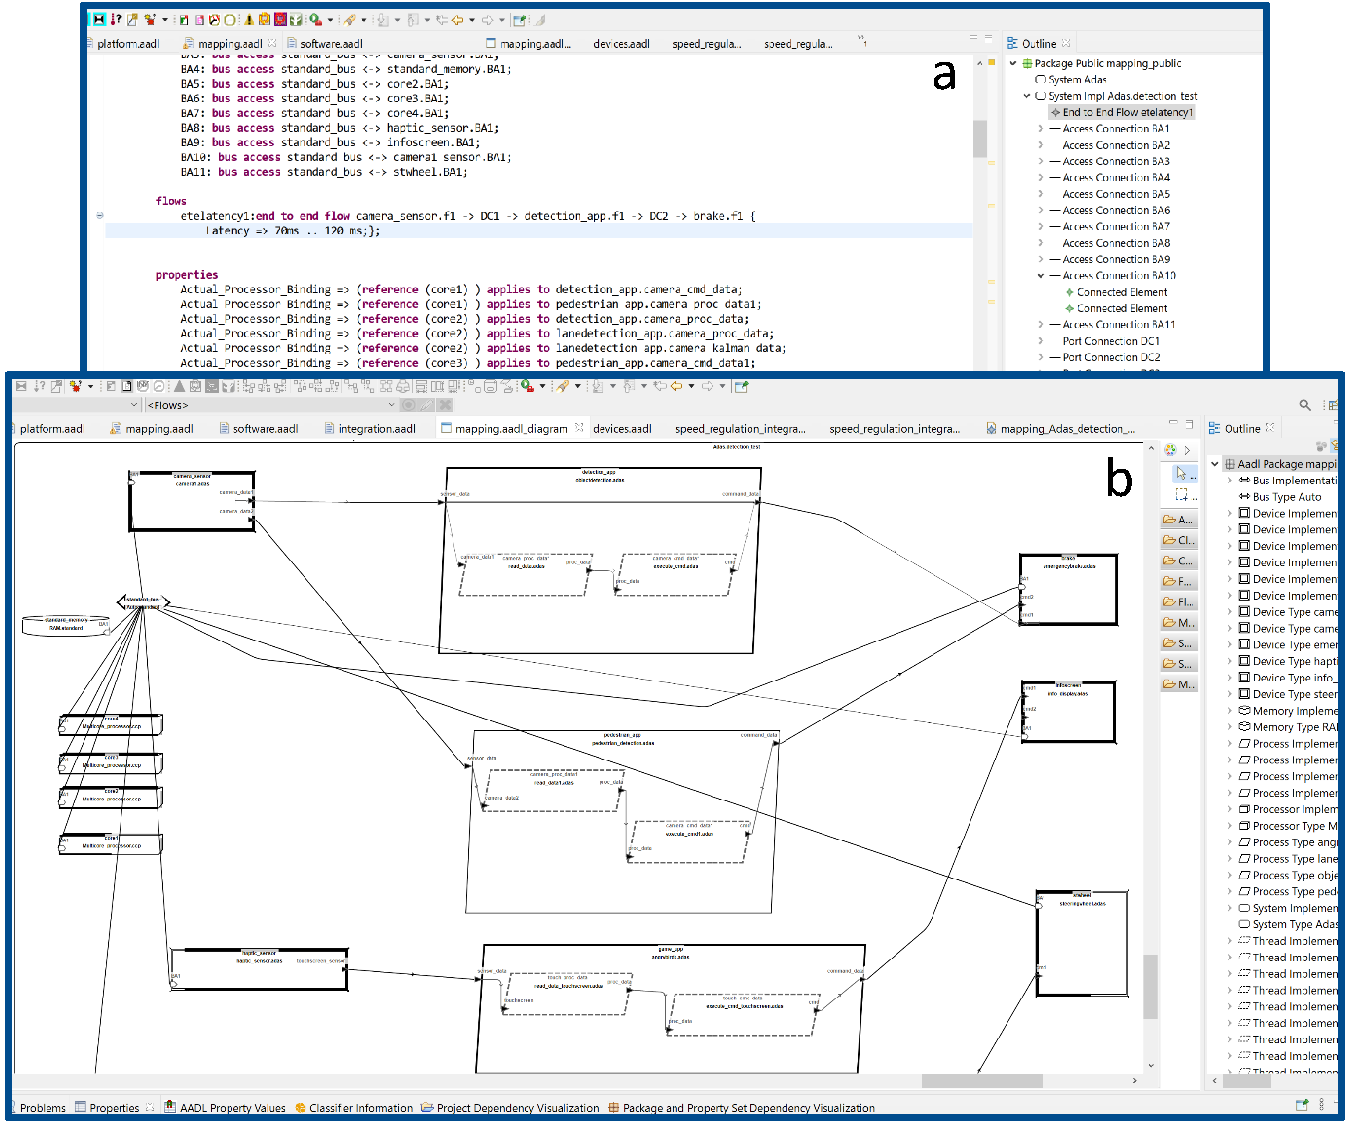
\includegraphics[width=\textwidth]{figures/osate_project.pdf}
\caption{ The AADL text editor (a) to synchronized graphical editor (b) in OSATE framework.}
\label{fig41}
\end{figure}


\subsection{Non-commercial/Open-source Frameworks}
 This subsection discusses non-commercial computer-aided tools to design and synthesize embedded and E/E systems. At the end of this subsection, an overview of this analysis is presented as a table, including details regarding each illustrated framework.
 
\subsubsection{OSATE (Open Source AADL Tool Environment)} 
%It is a powerful open-source tool that creates AADL (architecture analysis and design language) models using a syntax-aware text editor and synchronized graphical editor (See Figure. \ref{fig41}). OSATE is an Eclipse-based tool and comprises modeling elements for aerospace and the automotive systems using AADL language~\cite{feiler2019open},~\cite{osate}. 
It is a highly effective open-source tool for creating models using the architecture analysis and design language (AADL) with a syntax-aware text editor and a synchronized graphical editor (as seen in Figure \ref{fig41})\cite{askaripoor2022architecture}. OSATE is an Eclipse-based tool that provides modeling elements specifically designed for aerospace and automotive systems using the AADL language~\cite{feiler2019open},\cite{osate}.

\begin{figure}[ht]
\centering
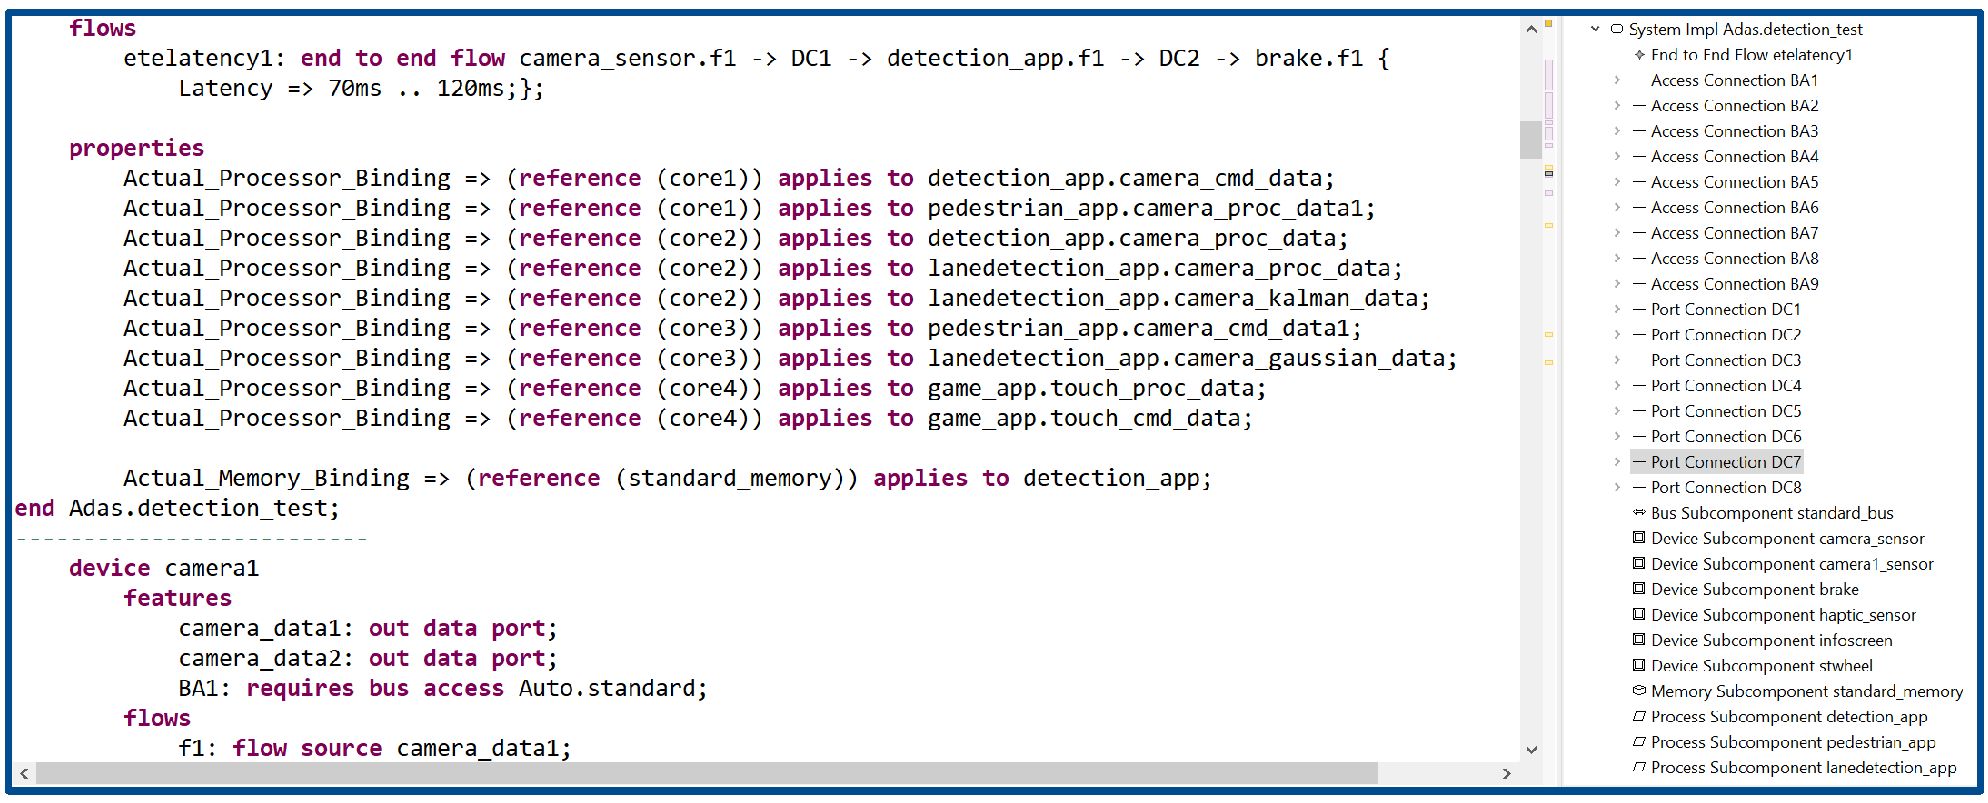
\includegraphics[width=1\textwidth]{figures/osateProject.pdf}
\caption{ The AADL text editor for a lane detection application including flow analysis, processor and memory bindings in OSATE framework.}
\label{fig042}
\end{figure}


\begin{figure}[ht]
\centering
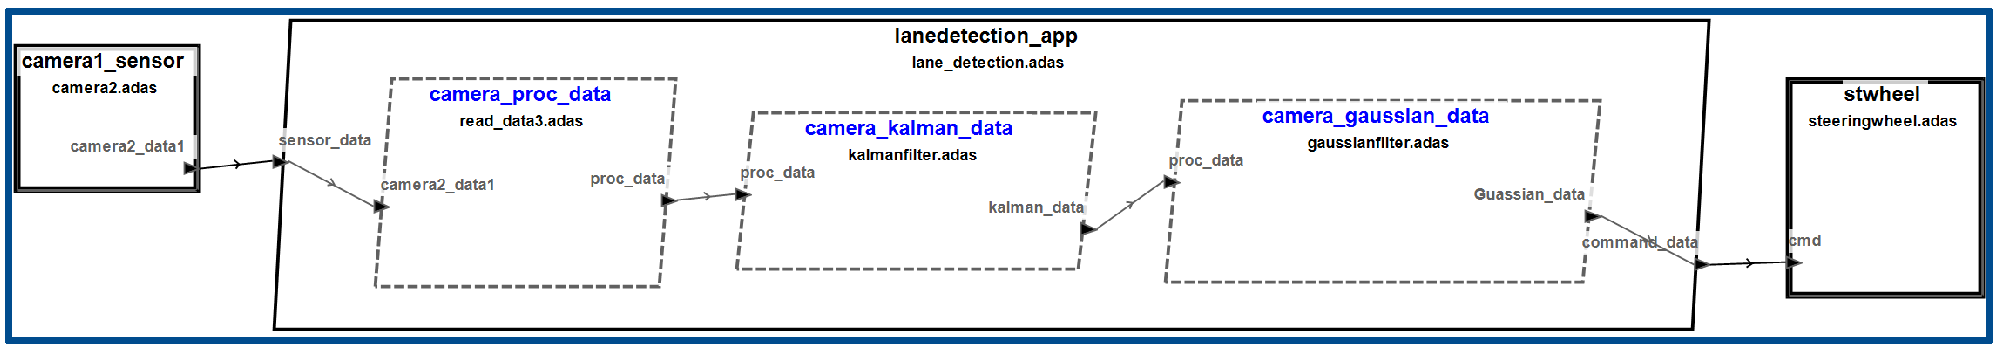
\includegraphics[width=1\textwidth]{figures/osateProject1.pdf}
\caption{ The synchronized graphical editor for a lane detection application created based on the AADL text in the OSATE framework.}
\label{fig0043}
\end{figure}

%AADL is a modeling language that supports early and repeated analyses of a system’s architecture concerning performance-critical properties through an extendable notation, a tool framework, and precisely specified semantics. The language utilizes formal modeling concepts for the description and analysis of application system architectures in terms of distinct components and their interactions.  It includes abstractions of software (e.g., process, and thread), computational hardware (e.g., processor, bus, device, and memory), and system components for  determining and analyzing automotive, aerospace, and real-time embedded systems, and investigating the performance capabilities of the designed system, for instance, data-flow analysis (i.e., collecting information about the set of values computed at different points in the designed model/system). Also, it provides mapping of software components (e.g., a process) into computational hardware elements, for example, a processor. AADL is especially effective for model-based analysis and specification of complex real-time embedded systems~\cite{feiler2006architecture}.
\begin{figure*}[ht]
\centering
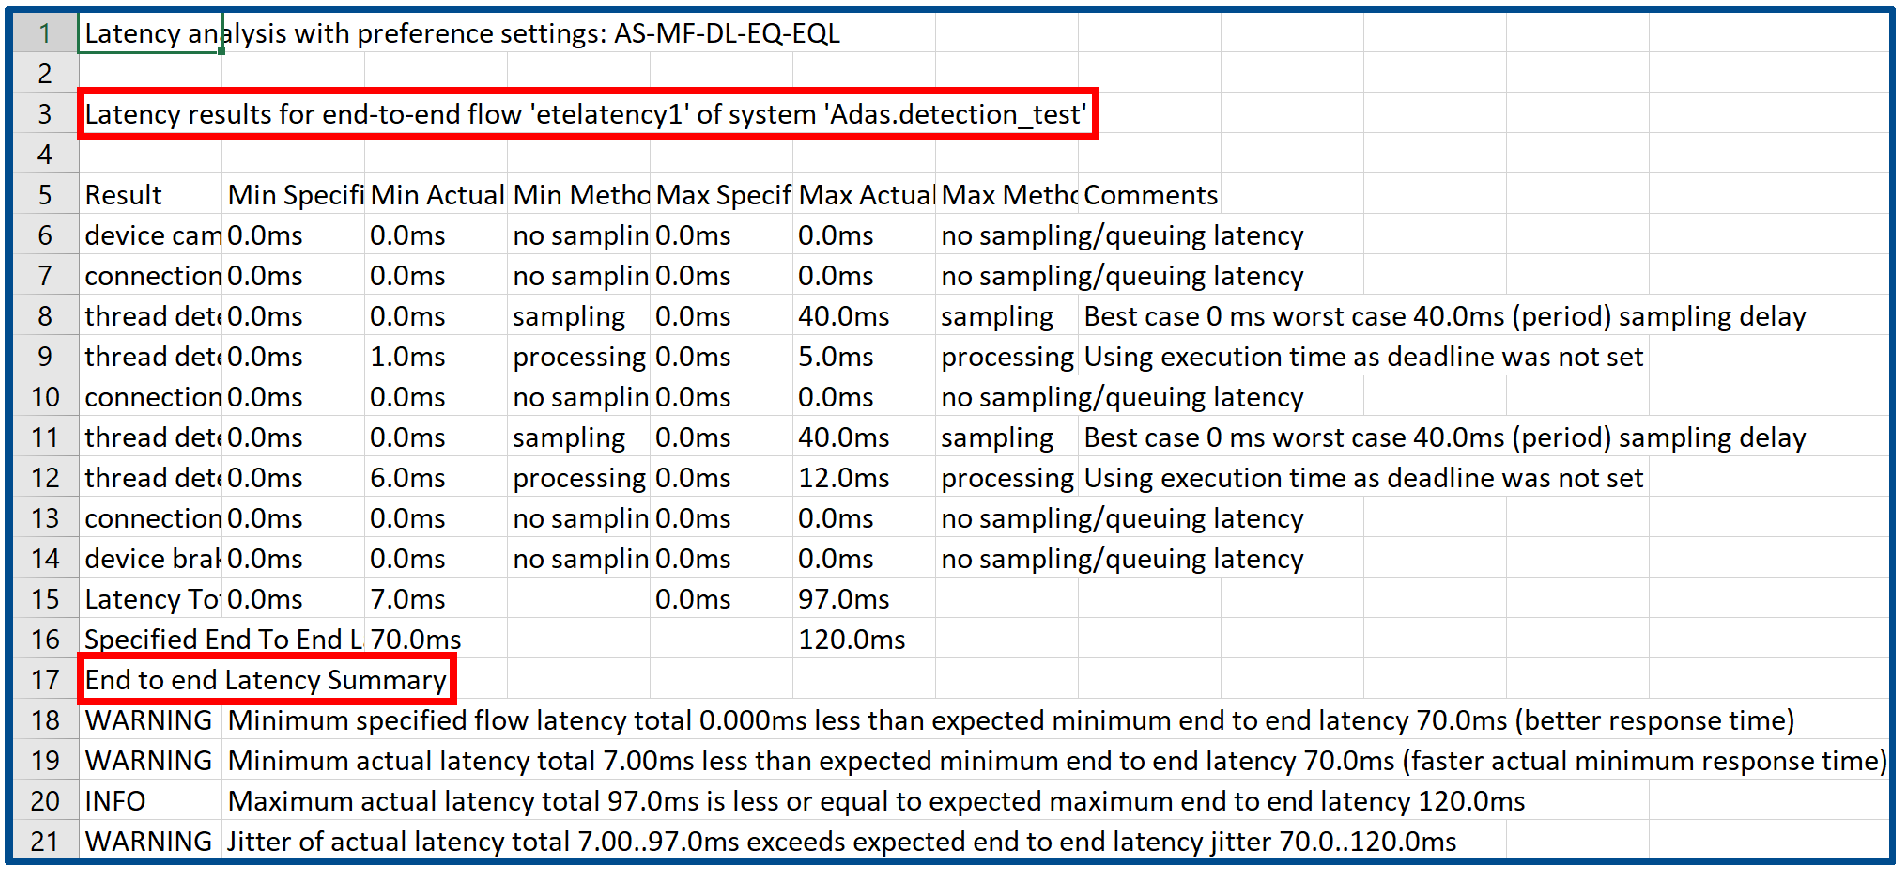
\includegraphics[width=1\textwidth]{figures/etelatency_osate.pdf}
\caption{ The report of end-to-end latency analysis for the specified flows in the OSATE tool.}
\label{fig045}
\end{figure*}


AADL is a versatile modeling language designed to provide early and recurrent assessments of system architecture with a focus on performance-critical properties. This is achieved through the use of a customizable notation, a comprehensive tool framework, and well-defined semantics. The language is based on formal modeling principles that allow for the characterization and examination of application system architectures through the identification of individual components and their interactions.
The scope of this includes abstract representations of software elements such as processes and threads, computational hardware, e.g., processors, buses, devices, and memory, and various system components. This is done with the aim of determining and analyzing automotive, aerospace, and real-time embedded systems, as well as examining the performance capabilities of the designed system through techniques like data-flow analysis. This involves collecting information about the set of values computed at different points within the designed model or system.
Additionally, the AADL facilitates the mapping of software components, such as processes, to computational hardware elements, such as processors. AADL has been proven to be particularly useful in the model-based analysis and specification of complex real-time embedded systems~\cite{feiler2006architecture}. 

For example, Figure~\ref{fig042} shows an AADL text for a lane detection application that takes flow analysis and processor bindings into account. Moreover, Figure~\ref{fig0043} presents the graphical visualization of the AADL text for the lane detection application.
\begin{figure}[hb!]
\centering
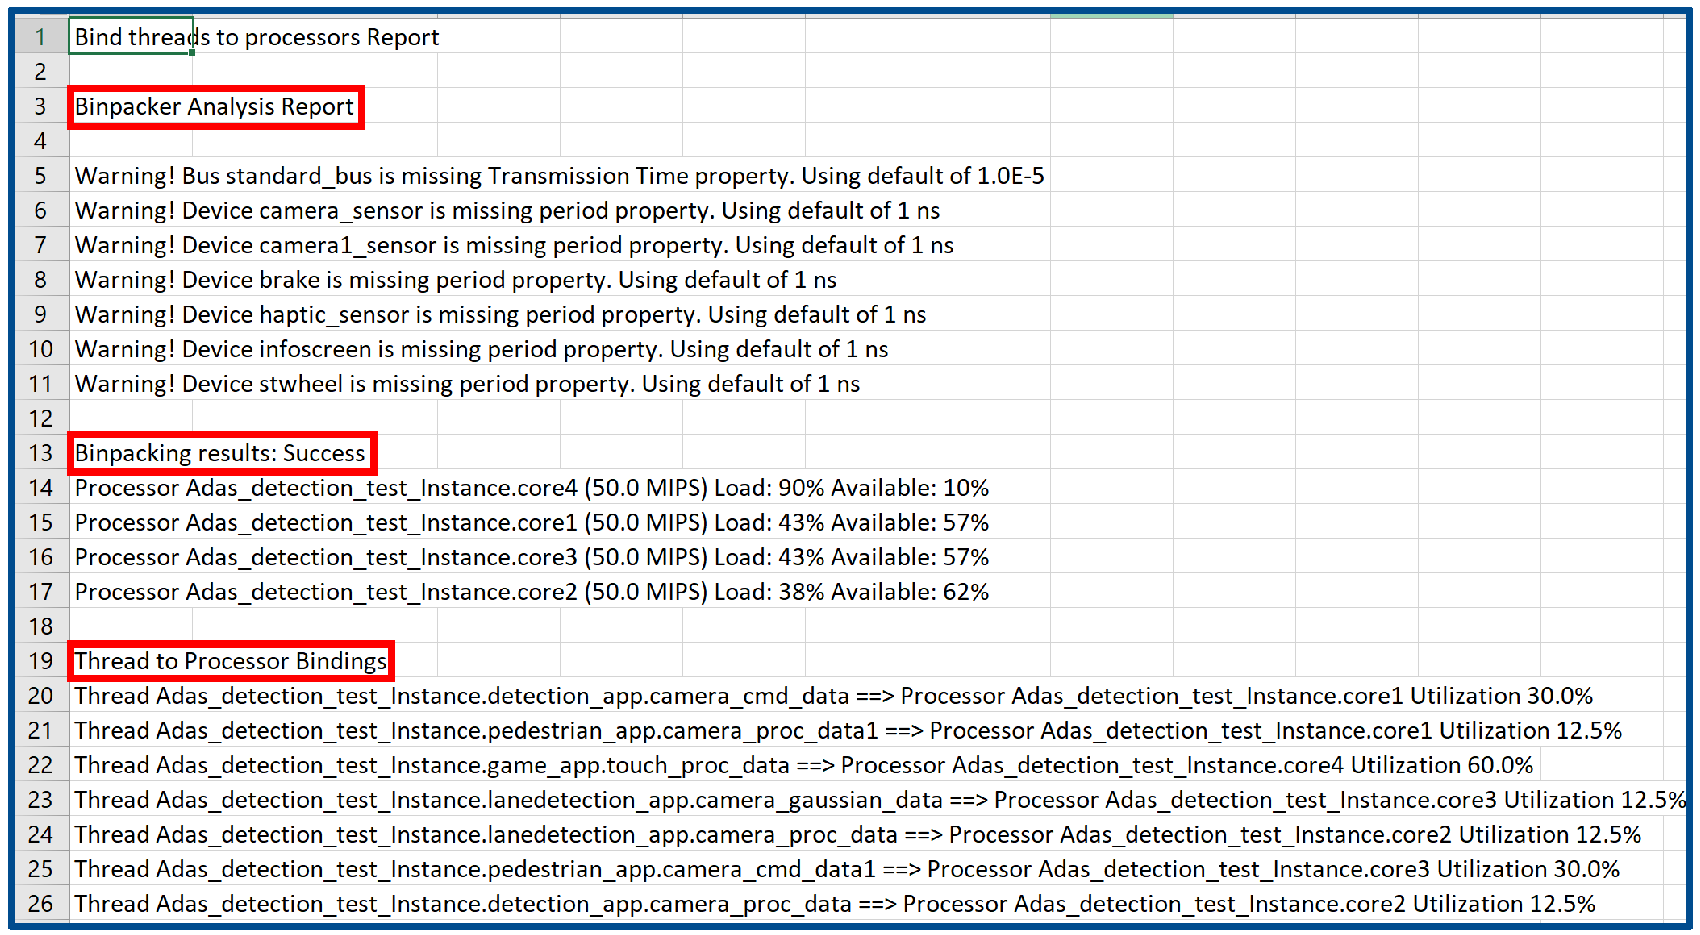
\includegraphics[width=1\textwidth]{figures/binpacking_osate.pdf}
\caption{Binpacking analysis and thread to processor bindings report in OSATE framework.}
\label{fig044}
\end{figure}

%By using the OSATE tool, the user can model a system (e.g., an ADAS system) including the hardware and software down to the application-level (See Figure.~\ref{fig41}). For instance, the threads used for each application can be modeled, including their properties such as period, compute execution time, million instruction per second (MIPS) budget, and reference processor. %The OSATE checks the model created by the user in terms of syntax issues regarding the AADL text and violations in properties definition for each specified component. 
The OSATE tool allows users to model a system, including both hardware and software components, down to the application level, as demonstrated in Figure~\ref{fig41}. With this tool, users can model the threads used for each application, specifying properties such as period, computation execution time, million instructions per second (MIPS) budget, and reference processor.
The OSATE verifies the model created by the user for syntax errors in the AADL text and property definition violations for each component specified.
%Moreover, various model analyses can be done by this framework comprising a flow latency check including end-to-end flow latency computation, scheduling analysis (such as scheduling bound threads, i.e., processor utilization report, binding and scheduling threads, i.e., thread binding report, and rate monotonic priority assignment), budget analysis (comprising analyzing bus load, power requirements, resource allocations, computer resource budgets, and calculating the total weight), and safety analysis comprising fault tree analysis (FTA), functional hazard assessment (FHA), fault impact analysis, failure mode effect analysis (FMEA), and checking unhandled faults.
In addition, this framework allows for a range of model analyses to be performed, including a flow latency check that computes the end-to-end flow latency. For example, Figure \ref{fig045} shows the latency results for the defined flows of a use case in the tool. 
This tool includes scheduling analysis such as scheduling bound threads, i.e., determining processor utilization as a report, binding and scheduling threads, i.e., thread binding report, and assigning rate monotonic priority. For instance, the binpacking analysis and also thread to processor bindings report for a specific use case generated by the OSATE are displayed in Figure \ref{fig044}. The OSATE also covers budget analysis that involves analyzing bus load, power requirements, resource allocations, computer resource budgets, and calculating the total weight. Moreover, the OSATE tool comprises safety analysis that incorporates fault tree analysis (FTA), functional hazard assessment (FHA), fault impact analysis, failure mode effect analysis (FMEA), and the identification of unhandled faults~\cite{osate,askaripoor2022architecture}.
%In addition, various semantic checks or functional integration analyses can be performed using this framework such as checking binding constraints, connection binding consistency, port connection consistency, etc. Also, this tool has different code generation capabilities utilizing various plugins, e.g., Ocarina, and is capable of importing models from MATLAB and Simulink into the OSATE~\cite{ocarina},~\cite{ocarinapaper},~\cite{MATLAB:2010}. 
Furthermore, this framework allows for the performance of a variety of semantic checks and functional integration analyses, including the examination of binding constraints, the consistency of connection bindings, and port connection consistency. This tool also boasts diverse code generation capabilities through the use of various plugins, such as Ocarina, and has the capability of importing models from both MATLAB and Simulink into the OSATE~\cite{ocarina,ocarinapaper,MATLAB:2010}.




%However, OSATE does not use or cover any DSE approaches, e.g., solving mapping problems for multi-core automotive computing units, and consequently, it supports no optimization~\cite{osate}. In addition, it covers a limited number of safety attributes as illustrated before. 

Despite its capabilities, the OSATE does not incorporate any DSE techniques, such as solving mapping problems for multi-core automotive computing units. As a result, it does not offer any optimization capabilities. Additionally, its coverage of safety attributes is limited as previously discussed~\cite{askaripoor2022architecture}.





\subsubsection{ArcheOpterix}
%As mentioned before, finding an acceptable architecture design is a challenging task for software and system architects, considering quality and functional requirements in the architecture design phase. %ArcheOpterix is an open-source Eclipse-based tool that contributes to simplifying the task using evaluation techniques, a DSE approach, and optimization heuristics for AADL specifications.
It was previously stated that determining a suitable architecture design is a difficult task for software and system architects, as they must take into account both quality and functional requirements during the design phase.
ArcheOpterix is a tool designed to make the task of evaluating, designing, and optimizing AADL specifications easier and more efficient. This open-source tool~\cite{aleti2009archeopterix}, which is based on the Eclipse platform, utilizes evaluation techniques, a DSE approach, and optimization heuristics to achieve its goals.
%The framework supports modeling of software components and communication among software components, ECUs, buses, and services. Moreover, the tool can optimize the deployment of software components to ECUs considering design constraints and optimization objectives, including redundancy allocation, and cost~\cite{aleti2009archeopterix}.
The framework in question provides the capability to model software components, as well as the communication between software components, ECUs, buses, and services. Moreover, the tool has the ability to optimize the deployment of software components to ECUs while considering design constraints and optimization objectives such as redundancy allocation and cost-effectiveness~\cite{aleti2009archeopterix}.







%This tool can specify the uncertain information relevant to system parameters and, therefore, search for the most optimal and robust candidate architecture. In addition, a list of the most appropriate optimization algorithms, comprising multi-objective genetic algorithm (MOGA), non-dominated sorting genetic algorithm (NSGA-II), pareto ant colony algorithm (P-ACO), simulated annealing (SA), Hill Climbing, bayesian heuristic for component deployment optimization (BHCDO), Random Search Algorithm, and Brute-Force Algorithms, can be provided by ArcheOpterix so that the user can choose the most suitable one~\cite{meedeniya2011reliability}.
The ArcheOpterix tool is designed to identify uncertain information related to system parameters and search for the optimal and robust candidate architecture. It also provides a list of the most appropriate optimization algorithms, including multi-objective genetic algorithm (MOGA), non-dominated sorting genetic algorithm (NSGA-II), pareto ant Colony algorithm (P-ACO), simulated annealing (SA), Hill Climbing, Bayesian Heuristic for component deployment optimization (BHCDO), Random Search Algorithm, and Brute-Force Algorithms, allowing the user to select the most suitable one~\cite{meedeniya2011reliability}.
\begin{figure*}[t]
\centering
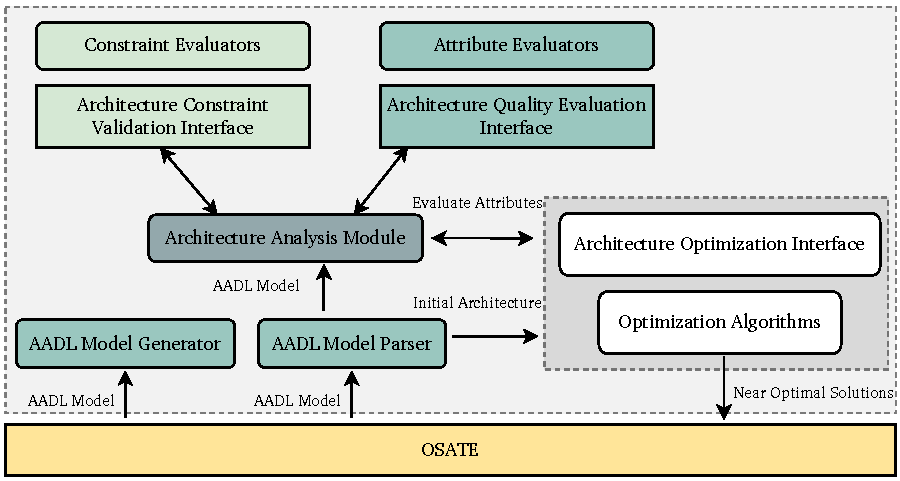
\includegraphics[width=\textwidth]{figures/Archeopterix_new.pdf}
\caption{The architecture of ArcheOpterix framework~\cite{askaripoor2023designer}.}
\label{fig046}
\end{figure*}
%Figure. \ref{fig046} shows the high-level architecture of the ArcheOpterix framework. As shown, it consists of various modules, of which the most important parts are explained in the following~\cite{meedeniya2011reliability}.  
As depicted in Figure \ref{fig046}, the high-level architecture of the ArcheOpterix framework comprises of multiple modules, the key components of which will be outlined below~\cite{meedeniya2011reliability}.


\begin{itemize}
    \item AADL Model Parser: %It interprets and extracts system descriptions from an AADL specification coming from the OSATE tool. The module can access AADL elements such as components, services, buses, etc. The extracted parameters are sent to the Architecture Analysis Module, as an input, which supports the two interfaces for analyzing the model comprising Architecture Constraints Validation and Architecture Quality Evaluation Interface (See Figure. \ref{fig4}).
    It is a module that is designed to interpret and extract information from an AADL specification generated by the OSATE tool. This module has the capability to access various AADL elements, such as components, services, and buses. The extracted parameters are then passed on to the Architecture Analysis Module as input, which provides support for two interfaces for analyzing the model, including the Architecture Constraints Validation Interface and the Architecture Quality Evaluation Interface (as illustrated in Figure \ref{fig046}).




    \item Architecture Constraints Validation Interface: %As displayed in Figure. \ref{fig4}, it provides a plug-in point for Constraint Evaluator modules that check a given architecture for constraint satisfaction.
     As illustrated in Figure \ref{fig046}, offers a connection point for the implementation of Constraint Evaluator modules that assess the compliance of a given architecture with established constraints.




    \item Architecture Quality Evaluation Interface: %In this part, various quality evaluation functions can be taken into account. In ArcheOpterix, the Attribute Evaluator module performs quality evaluation functions, which can be extended for evaluated features. Current integrated features in ArcheOpterix are Service Reliability, Data Transmission Reliability, and Communication Overhead.
    In this part, a variety of quality evaluation functions can be considered. The Attribute Evaluator module in ArcheOpterix performs these evaluation functions, which can be expanded to include additional evaluated features. Currently, ArcheOpterix includes the evaluation of Service Reliability, Data Transmission Reliability, and Communication Overhead as integrated features.




\item Architecture Optimization Interface: %It provides an opportunity to add new optimization algorithms to the framework. The current tool comprises Exact Algorithms, Genetic Algorithms, and Ant Colony Optimization~\cite{meedeniya2011reliability}.
The current framework offers the possibility of incorporating new optimization algorithms. The tool currently includes Exact Algorithms, Genetic Algorithms, and Ant Colony Optimization~\cite{meedeniya2011reliability}.

\end{itemize}


%However, this tool has several limitations in the context of mapping, architecture synthesis, and software integration for automotive platforms. %First of all, the framework is outdated and also is not well-documented for use. It does not support mapping analysis and solving the mapping problem for multi-core architecture, and there is no focus on multi-core computing platforms for automotive applications.%In addition, the safety-related attributes regarding ISO 26262, are not covered in this tool except for reliability, and the framework itself supports no model checking and model analysis. Also, the covered optimization objectives by ArcheOpterix are restricted, including cost, communication overhead, and data transmission reliability; furthermore, the tool has a limited number of architectural elements.

Despite its usefulness, this tool has several limitations when it comes to mapping, architecture synthesis, and software integration for automotive platforms.
Initially, the framework is outdated and lacks proper documentation for usage. It does not provide support for mapping analysis or solving mapping problems for multi-core architectures and does not place a focus on multi-core computing platforms for automotive applications.
Moreover, the safety attributes specified in ISO 26262, excluding reliability, are not incorporated in this tool. Additionally, the framework itself does not have any model checking or model analysis capabilities. The optimization objectives covered by ArcheOpterix are limited to cost, communication overhead, and data transmission reliability. Furthermore, the tool has a limited set of architectural elements~\cite{askaripoor2022architecture}.





\subsubsection{PerOpteryx} %It is another open-source framework for feature configuration and clustering during the design stage in the software domain.Authors in~\cite{koziolek2011peropteryx} claimed that this approach can contribute to finding optimal solutions for software architecture based on predefined requirements and constraints while applying multi-objective evolutionary optimization to software architectures modeled with the Palladio Component Model. In such a case, software architects can select the most suitable architecture for their situation.This approach provides software architecture solutions based on different quality attributes such as performance, cost, and reliability using the DSE method. 
Another open-source framework exists for feature configuration and clustering during the design phase within the software domain, as described by the authors in~\cite{koziolek2011peropteryx}. They assert that this approach can lead to finding the optimal solutions for software architecture, taking into consideration the predefined requirements and constraints, by utilizing multi-objective evolutionary optimization on software architectures modeled using the Palladio Component Model. With this approach, software architects have the ability to choose the most appropriate architecture for their specific circumstances.
The proposed methodology offers software architectural solutions that are optimized based on various quality attributes, including performance, cost, and reliability, utilizing the DSE technique.
%PerOpteryx automatically creates architecture candidates based on several degrees of freedom of component-based software architectures and afterward evaluates and optimizes these architecture candidates according to the specified requirements. This approach was validated by applying two different architecture models comprising a business reporting system and an industrial control system~\cite{busch2019peropteryx}.
PerOpteryx is a tool that generates potential software architecture candidates based on various degrees of freedom in component-based software architectures. Afterward, these candidates are evaluated and optimized to meet the specified requirements. The effectiveness of this approach was demonstrated through the application of two different architecture models, including a business reporting system and an industrial control system~\cite{busch2019peropteryx}.


%However, this framework has no support for mapping analysis or DSE approach for task mapping i.e., finding a mapping solution for assigning, e.g., processes into cores integrated into automotive high-performance computing units, as meeting all safety and non-safety requirements. Also, it has limited elements which can be used in the software architecture, and there is no model checking or analysis integrated into this approach. More importantly, automotive safety parameters have not been defined in this open-source framework, and PerOpteryx is outdated and suffers from a lack of proper documentation.
However, this framework lacks support for mapping analysis or a DSE approach for task mapping, meaning it cannot find a solution for assigning processes, such as those integrated into automotive high-performance computing units, to cores while meeting all safety and non-safety requirements. Additionally, the framework has limited elements for use in the software architecture and does not include any model checking or analysis. Furthermore, the open-source framework does not define automotive safety parameters, and the PerOpteryx tool is outdated and suffers from inadequate documentation.








\subsubsection{MechatronicUML} %As far as modern technical systems are elaborate, including reconfigurable mechatronic systems where most control and reconfiguration functionality is identified in the software, several requirements have to be satisfied to apply the model-driven development approach to these types of systems.%Therefore, an open-source framework, based on the Eclipse framework, to model software/hardware components, define constraints, and verify the defined models, comprising the constraints using a model checker, namely UPPAAL, for the embedded systems is presented in~\cite{behrmann2006uppaal},~\cite{burmester2004model}. 
Due to the complex nature of modern technical systems, particularly reconfigurable mechatronic systems where most control and reconfiguration functionality is embedded in software, it is necessary to meet specific requirements in order to effectively utilize a model-driven development approach for these types of systems.
Consequently, a research paper presented an open-source framework, built on the Eclipse framework, for modeling software and hardware components, specifying constraints, and verifying the models through the use of a model checker called UPPAAL for embedded systems. This framework is described in~\cite{behrmann2006uppaal},~\cite{burmester2004model}.

%This tool is a model-based approach and tries to bring model-based design formal analysis to the mechatronic domain. This tool supports the DSE approach to find the solution based on predefined constraints in the model; moreover, it provides software reconfiguration in such a way that this function allows the user to design a system so that the system adapts automatically at runtime according to the changing environment. 
This tool is an innovative model-based approach that aims to bring the benefits of model-based design and formal analysis to the field of mechatronics. By utilizing a DSE approach, it helps users to find solutions based on predefined constraints in the model. Furthermore, it offers software reconfiguration capabilities that allow for automatic adaptation of the system at runtime to accommodate changes in the environment, providing the user with greater flexibility in the design process.
%This framework has the capability of C code generation, and the designed models can be simulated using MATLAB Simulink, Modelica, or the Functional Mock-up Interface (FMI)~\cite{fritzson1998modelica},~\cite{MATLAB:2010},~\cite{schafer2010model}.  
This framework possesses the ability to generate code in the C programming language, and the models created can be simulated through the use of MATLAB Simulink, Modelica, or the functional mock-up interface (FMI)\cite{fritzson1998modelica},\cite{MATLAB:2010},\cite{schafer2010model}.
%, this tool has limitations based on our criteria for mapping and software integration in the automotive domain. Firstly, mapping analysis and DSE related to mapping problem in computing units are not covered by this framework, and MechatronicUML supports no optimization. Furthermore, no safety-related attributes were considered in this tool for modeling, analysis, and solving, and this approach does not focus on multi-core or high-performance computing unit modeling and analysis. In addition, this tool is not updated and has no active community or proper documentation.

Nonetheless, the limitations of this tool must be acknowledged based on the criteria set for mapping and software integration within the automotive industry. Firstly, the framework does not address mapping analysis or DSE related to mapping problems in computing units, and MechatronicUML does not provide optimization capabilities. Furthermore, the tool does not take into consideration safety-related attributes for modeling, analysis, and problem-solving purposes. Additionally, this tool is outdated and lacks an active community or proper documentation.

\begin{figure}[ht]
\centering
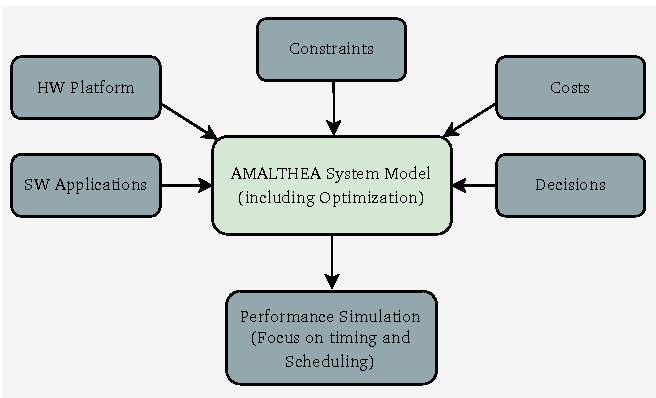
\includegraphics[width= 0.85\textwidth]{figures/amalthea_approach1.pdf}
\caption{The APP4MC architecture~\cite{askaripoor2023designer}.}
\label{fig06}
\end{figure}


\subsubsection{App4MC} %As mentioned before, the automotive industry increasingly utilizes multi- and many-core systems to deal with ADAS and self-driving functionalities because of a considerable number of applications that require high computational power for processing. 
As previously mentioned, the automotive industry has increasingly adopted the use of multi-core and many-core systems to manage ADAS and autonomous driving functionalities due to the significant number of applications that require a high level of computational power for processing.
%APP4MC is anopen-source Eclipse platform that concentrates on performance simulation regarding mostly scheduling and timing analysis in multi-core platforms using a model-based development approach (See Figure. \ref{fig6})~\cite{hottger2015model},~\cite{hottger2017app4mc}. 
APP4MC is an open-source Eclipse platform that focuses on the performance simulation of scheduling and timing analysis in multi-core platforms. This platform utilizes a model-based development approach, as shown in Figure~\ref{fig06}. It is dedicated to providing insights into the performance of multi-core systems~\cite{hottger2015model,hottger2017app4mc}.
%The hardware and software elements can be modeled, including different properties such as the processor type, connection type among various specified modules, OS schedulers, and task properties such as execution time and deadline. In addition, different timing constraints with respect to the tasks, OS schedulers, and mapping constraints (i.e., assigning tasks and schedulers to a specific core) can be defined, visualized, checked, and finally validated using this tool. 
The hardware and software components can be modeled, including specific properties like the processor type, connections between various modules, OS schedulers, and task properties such as execution time and deadline. Furthermore, different timing constraints related to the tasks, OS schedulers, and mapping constraints (i.e. the assignment of tasks and schedulers to a specific core) can be defined, visualized, verified, and validated using this tool.
%   \mynotes{too much space and low information content. It is also far from its explanation in the text. As I see there are two images describing APP4MC. It gives me the impression that it is much more important/relevant technology in comparison to others. Right? If No, the we may shorten it...}
\begin{figure}[ht]
\centering
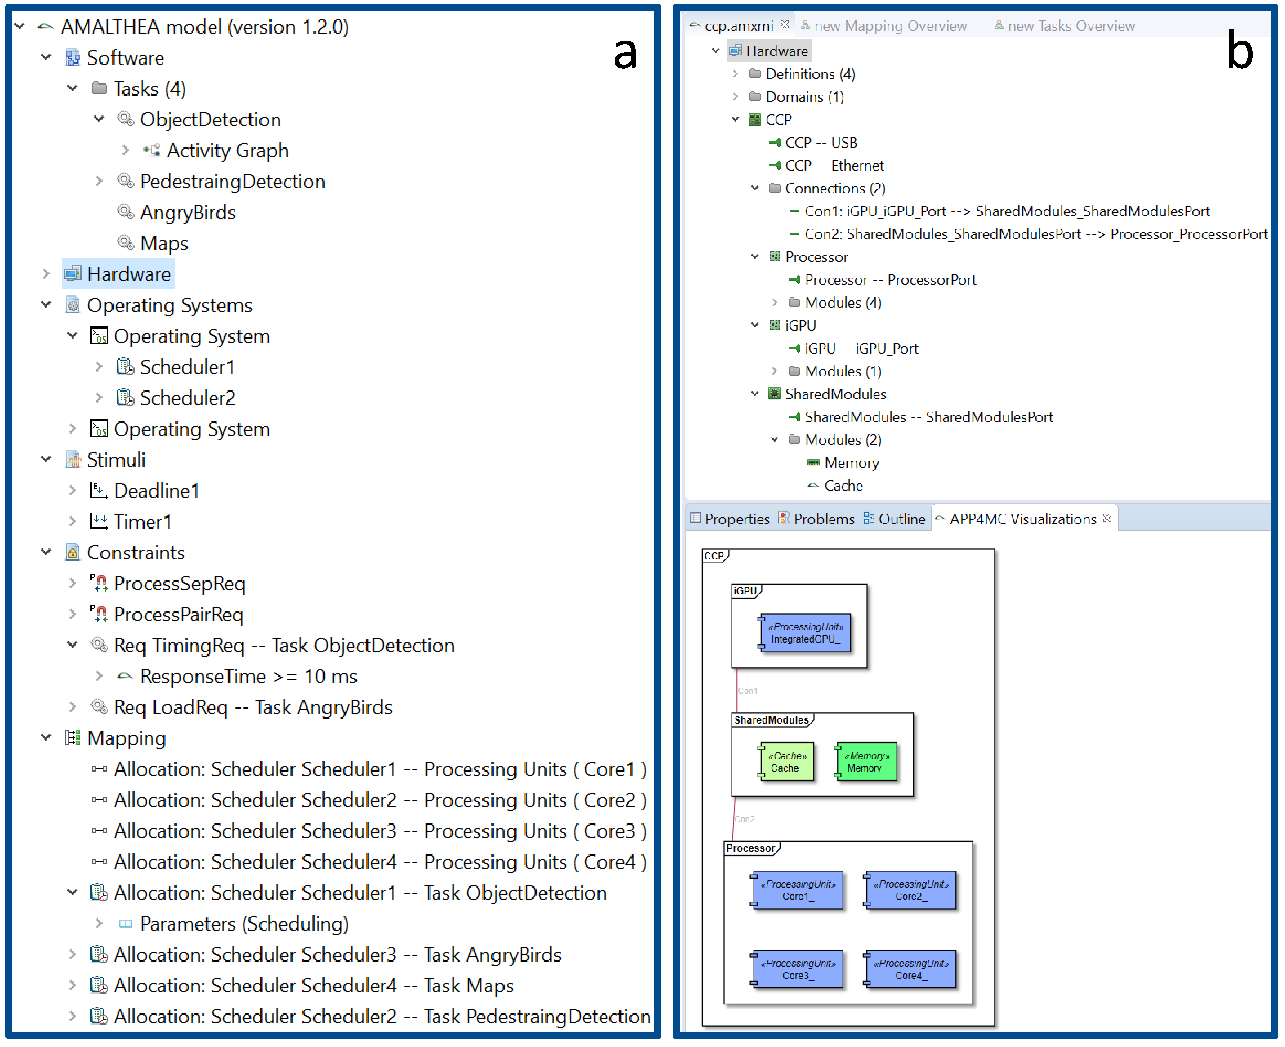
\includegraphics[width= \columnwidth]{source/app4mc11_cropped.pdf}
\caption{A model of the hardware and software system in the automotive industry has been developed using the APP4MC framework. This model encompasses timing and mapping constraints (a) and includes a visual representation of the hardware model (b)~\cite{askaripoor2022architecture}.}
\label{fig66}
\end{figure}
%Moreover, the definition of the hardware and software model and constraints and the whole model can be simulated (i.e., using different graphs e.g, Gantt chart and tables to present the result) while considering different optimization goals comprising load balancing, energy consumption, and memory mapping. 

In addition, the hardware and software model, as well as its constraints, can be defined and simulated by utilizing various visual aids such as graphs (e.g., Gantt chart) and tables to present the results. This simulation takes into account different optimization goals, including load balancing, energy consumption, and memory mapping.
%Figure~\ref{fig66} shows an example of a modeled automotive system in APP4MC including tasks, hardware, OS, Stimuli, constraints, and mapping. For instance, in the mapping part, schedulers can be assigned to the cores and tasks (See Figure~\ref{fig66} (a)). In Figure~\ref{fig66} (b) the hardware model, including a processor (comprising four cores), integrated GPU (iGPU), shared modules such as cache and memory, and communication among these components, is visualized using the AAP4MC visualization feature. 
Figure~\ref{fig66} illustrates a modeled automotive system within APP4MC that includes components such as tasks, hardware, operating system, stimuli, constraints, and mapping. For example, the mapping section of the model allows schedulers to be assigned to cores and tasks, as depicted in Figure~\ref{fig66} (a). In Figure~\ref{fig66} (b), the hardware model, which includes a processor with four cores, an integrated GPU (iGPU), shared modules such as cache and memory, and communication between these components, is visualized using the visualization feature of AAP4MC~\cite{askaripoor2022architecture}.




%However, this framework does not contribute to automating the mapping of various tasks to various HW elements, for instance, core, including the safety and non-safety requirements (i.e., DSE for mapping problem). APP4MC only analyzes and simulates the task mapping but not solving. Furthermore, it is limited in the covered safety attributes and optimization goals and there are a considerable number of E/E architecture elements which are not considered by AAP4MC. 
However, the APP4MC framework has limitations when it comes to automating the mapping of tasks to hardware elements such as cores, taking into account both safety and non-safety requirements (i.e. the task mapping problem using DSE). While it provides analysis and simulation of task mapping, it does not provide a solution. Moreover, it has limited coverage of safety attributes and optimization goals, and a significant number of E/E architecture elements are not considered in the framework~\cite{askaripoor2022architecture}.



\subsubsection{Autofocus3}
%Another open-source and Eclipse-based tool uses a model-based development approach to synthesize E/E architectures. This framework supports architecture modeling from requirements to code generation for embedded systems. Additionally, the tool can simulate the designed model including its defined constraints and check and validate the model. 
Another open-source tool that is based on the Eclipse platform utilizes a model-based development approach to synthesize E/E architectures. This framework supports the modeling of architecture, starting from requirements all the way to the generation of code for embedded systems. Furthermore, the tool is equipped with the capability to simulate the designed model, including the defined constraints, and to perform checks and validate the model.
%It utilizes domain-specific modeling language to formalize an exploration problem and is capable of calculating end-to-end latency and schedule synthesis using the DSE method; moreover, optimization algorithms, such as binary search, have been integrated into this tool to apply the defined optimization objectives, including timing and communication load, to the explored solution~\cite{aravantinos2015autofocus,voss2014design,holzl200713}.
The tool employs a domain-specific modeling language to formalize exploration problems and has the capability to determine end-to-end latency and schedule synthesis through the use of the DSE method. Additionally, optimization algorithms such as binary search have been integrated into the tool to apply defined optimization objectives, such as timing and communication load, to the solution that is explored~\cite{aravantinos2015autofocus,voss2014design,holzl200713}.


 %Autofocus3 does not cover the solving approach for the mapping problem in the multi-core platforms considering functional and non-functional requirements to automate mapping configuration and there is no mapping analysis for these platforms. In addition, it supports a limited number of safety attributes, only ASIL level, and optimization goals for E/E architecture synthesis~\cite{askaripoor2022architecture}. 
 
 
 Autofocus3 falls short in addressing the issue of mapping configuration automation on multi-core platforms, taking into consideration both functional and non-functional requirements. There is also a lack of mapping analysis for these platforms. Moreover, it only offers limited support for safety attributes, specifically the ASIL level, and for the optimization goals related to the synthesis of the electronic and electrical architecture~\cite{askaripoor2022architecture}.


 \subsubsection{Clafer} 
%An approach that combines structural modeling with behavioral formalism to contribute to the mapping of feature configurations to component configurations or model templates. Calfer allows capturing feature models (variability), component models, and discrete control models (automata) in a single unified syntax and semantics. 
A methodology has been developed that combines structural modeling with behavioral formalism to aid in the mapping of feature configurations to component configurations or model templates. This approach, known as Calfer, allows for the integration of feature models (representing variability), component models, and discrete control models (in the form of automata) into a single, unified syntax and semantic framework.
%The language part is built on top of first-order logic with quantifiers over basic entities (for modeling structures) combined with linear temporal logic (for modeling behavior). This approach does DSE for feature modeling considering timing as a problem attribute, and it supports model analysis. Furthermore, it covers multi-objective optimization for the discovered solution comprising mass, end-to-end latency, and cost~\cite{juodisius2018clafer}.%~\cite{ross2019synthesis}.
The language component is constructed using a combination of first-order logic with quantifiers for modeling structures and linear temporal logic for modeling behavior. This approach engages in DSE with a focus on timing as an attribute, and it allows for model analysis. Additionally, it provides multi-objective optimization for the discovered solution by considering factors such as mass, end-to-end latency, and cost~\cite{juodisius2018clafer, ross2019synthesis}.

%However, Clafer supports no model checking, mapping analysis, or DSE for mapping problems in the embedded systems. The architectural elements are limited; moreover, there are no safety-related attributes covered by Clafer for model analysis. Besides, this approach has not given any considerations to the modeling and analysis of multi-core computing units. Furthermore, this approach is not well-documented and is outdated.  
Despite its potential, Clafer lacks certain important features for modeling and analysis in embedded systems. Specifically, it does not offer model checking, mapping analysis, or DSE for mapping problems. Additionally, the architectural elements in Clafer are limited and do not include safety-related attributes for model analysis. Furthermore, this approach has not taken into account the modeling and analysis of multi-core computing units. To add, the available information on this approach is not extensive and outdated~\cite{askaripoor2022architecture}.





\subsubsection{AAOL Framework}
%This model-based approach is a constraint-based E/E architecture optimization framework utilizing a domain-specific language. The supporting tool uses the DSE method to find the optimal solution for deployment problem considering design constraints, e.g., memory capacity and applying multi-objective optimization mechanism, and the applied goals are cost and weight~\cite{kugele2015deployment}.%~\cite{kugele2014model}. 
The model-based approach is a framework for optimizing E/E architecture using a constraint-based methodology and a domain-specific language. The accompanying tool leverages the DSE method to determine the optimal solution for the deployment problem while considering design constraints such as memory capacity, and it implements a multi-objective optimization mechanism with cost and weight as the defined objectives~\cite{kugele2015deployment, kugele2014model}.




%However, this tool has several limitations. It is limited in architectural elements regarding software and hardware level, e.g.,  it does not define any software application parameter. It covers no DSE for mapping problem in multi-core computing units, and it supports no model analysis and checking. In addition, it only takes ASIL level as a safety-related parameter into account for architecture synthesis, and it only covers a few optimization objectives. Also, this tool is outdated and is not well documented.

However, this tool has several limitations that hinder its full potential. In terms of architectural elements at the software and hardware level, it lacks a definition of software application parameters and does not address mapping problems in multi-core computing units. Furthermore, it lacks support for model analysis and checking. The tool only considers the ASIL as a safety-related parameter in architecture synthesis and only covers a limited number of optimization objectives. Furthermore, this tool is outdated and lacks comprehensive documentation~\cite{askaripoor2022architecture}.



\subsubsection{Assist}
%Aviation electronics (avionics) are sophisticated and distributed systems aboard an airplane. The complexity of these systems is continuously growing as an increasing number of functionalities are realized in software. Using multi-core processors allows multiple functions in one hardware while meeting all safety requirements, which results in performance improvement of the system which can be a significant breakthrough in the aviation industry. 
The aviation electronics, or avionics, used aboard airplanes are complex and highly distributed systems. With the constant addition of new functionalities in software, the complexity of these systems continues to increase. The use of multi-core processors enables multiple functions to be performed on a single hardware unit while still meeting all safety requirements, resulting in improved system performance. This represents a major advancement in the aviation industry.
%A model-based approach was introduced in~\cite{hilbrich2013deploying}, namely Assist, to solve and optimize mapping problems (i.e., deployment of a safety-critical application on the avionics hardware) for distributed systems in the aviation domain. It uses the DSE mechanism to find optimal mapping solutions while considering optimizations objectives, including resource usage, weight, and cost. In addition, this Eclipse-based tool can create a periodic schedule for real-time tasks and ensure a deterministic timing behavior~\cite{hilbrich2017experiences}.
A model-based solution, named Assist, is introduced in~\cite{hilbrich2013deploying} to address mapping problems and optimize deployment of safety-critical applications on avionics hardware in distributed systems within the aviation domain. The approach employs a DSE mechanism to determine optimal mapping solutions while taking into account optimization objectives, such as resource usage, weight, and cost. Furthermore, the Eclipse-based tool has the capability to generate a periodic schedule for real-time tasks and ensure a deterministic timing behavior~\cite{hilbrich2017experiences}.

%This framework, however, has some limitations. The specified architectural elements are extremely limited in terms of hardware and software level, and also its focus is on the aviation domain rather than automotive and E/E architecture. Moreover, it only supports redundancy as a safety-relevant attributes based on ISO 26262 for mapping problem. Also, Assist does not support model checking and model analysis, and the number of defined optimization goals is limited.

Despite its benefits, this framework has certain limitations that must be taken into consideration. Firstly, the hardware and software level of the specified architectural elements are quite restricted, and its primary focus is on the aviation domain, rather than the automotive and E/E architecture. Secondly, it only takes into account redundancy as a safety-relevant attribute based on ISO 26262 for mapping purposes, and does not provide support for model checking and analysis. Lastly, the number of defined optimization goals is limited~\cite{askaripoor2022architecture}.




\subsubsection{Deepcompass Framework}
%Designing embedded systems for multiprocessor platforms requires early prediction and the balancing of multiple system quality attributes. The authors of \cite{bondarev2007exploring} present a DSE framework for component-based software systems that allows an architect to gain insight into a space of possible design alternatives with further evaluation and comparison of these alternatives. This framework supports the design of multiple alternatives for software and hardware architectures, and it is capable of performing model analysis, mapping analysis, and model validation. 
The design of embedded systems for multi-processor platforms necessitates the prediction and balance of multiple system quality attributes at an early stage. In \cite{bondarev2007exploring}, a DSE framework is introduced for component-based software systems that provides architects with a means to explore a range of possible design options and evaluate and compare these alternatives. This framework facilitates the creation of multiple alternatives for both software and hardware architectures, and is equipped with the ability to conduct model analysis, mapping analysis, and model validation.
%Besides, it uses the DSE approach for finding the suitable SW/HW architecture alternatives while taking multiple optimization goals into account, comprising cost, throughput, and resource utilization.
Additionally, the tool employs a DSE method to determine the optimal software/hardware architecture options while considering multiple optimization objectives, including cost, throughput, and resource utilization.

%Nonetheless, it covers no automotive-related elements and multi-core computing units attributes. In addition, there is no DSE for the mapping problem, and it does not include any safety-related attributes. Also, the specified optimization goals are extremely limited. This open-source tool is outdated and is not well documented.   

However, it lacks any automotive-related elements and multi-core computing unit attributes and does not incorporate a DSE for the mapping problem. It also lacks any considerations for safety-related attributes, and the specified optimization goals are severely limited. Moreover, this open-source tool is outdated and lacks proper documentation~\cite{askaripoor2022architecture}.

\subsubsection{SCALL} 
%This is a prototype tool that uses an allocation method to provide deployment solutions for system architects in the design phase using DSE~\cite{vsvogor2015scall}. In addition, it supports multi-objective DSE, including heterogeneous component allocation, bandwidth, and communication cost, by utilizing heuristics and AHP approaches to support systems architects in complex allocation decisions in early design stages.
The prototype tool described here utilizes an allocation method to provide deployment solutions for system architects during the design phase by leveraging the concept of DSE~\cite{vsvogor2015scall}. It also supports multi-objective DSE, which encompasses the allocation of heterogeneous components, the optimization of bandwidth, and the minimization of communication cost. To assist system architects in making complex allocation decisions during the early design stages, the tool incorporates both heuristics and analytic hierarchy process (AHP) approaches.

%However, this approach does not consider model analysis, model checking, or mapping analysis. Also, there is no coverage regarding DSE for mapping problem in multi-core computing units and no safety-relevant constraints and requirements, and the automotive architectural elements have not been defined in this framework. Moreover, it does no optimization and is an outdated tool.
Despite these advancements, the current approach lacks consideration for model analysis, model checking, or mapping analysis. There is also no coverage of DSE for mapping problems in multi-core computing units and no provisions for safety-related constraints and requirements. Furthermore, the automotive architectural elements have not been clearly defined within this framework, and it lacks any optimization capabilities, rendering it outdated~\cite{askaripoor2022architecture}.


\begin{figure}[ht]
\centering
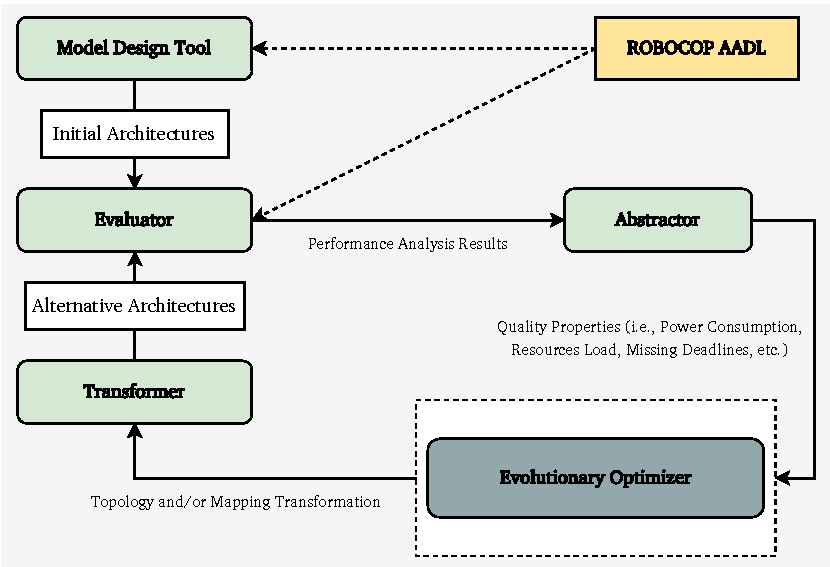
\includegraphics[width=0.8\columnwidth]{figures/Aqosa_framework.pdf}
\caption{The working scheme of the AQOSA toolkit~\cite{askaripoor2022architecture}.}
\label{fig07}
\end{figure}

\subsubsection{AQOSA}
%The authors in ~\cite{li2011evolutionary} introduceAQOSA (Automated Quality-driven Optimization of SoftwareArchitecture) toolkit to facilitate the design of software architecture in advanced component-based software development. It integrates modeling technologies,performance analysis techniques, and advanced evolutionarymulti-objective optimization algorithms to improve non-functional properties of systems in an automated manner. It enables the modeling of software components and the mapping of feature configurations to component configurations or model templates. 
Authors in ~\cite{li2011evolutionary} present the automated quality-driven optimization of software architecture (AQOSA)  toolkit as a solution for improving the design process of software architecture in advanced component-based software development. AQOSA integrates various technologies, including modeling techniques, performance analysis methods, and advanced evolutionary multi-objective optimization algorithms to automate the improvement of non-functional properties in software systems. The toolkit enables the modeling of software components and maps feature configurations to component configurations or model templates, thereby streamlining the design process.
%Additionally, it supports the DSE method, including multi-objective optimization (such as data flow latency, processor usage, and architecture cost), and the architect can easily design the initial architecture in OSATE~\cite{osate} utilizing AADL language~\cite{feiler2006architecture} and then import it into AQOSA framework. For software architecture modeling, AQOSA integrates ROBOCOP~\cite{bondarev2006process} (Robust Open Component-Based Software Architecture for Configurable Devices Project) modeling language (See Figure.~\ref{fig7}). 
Furthermore, the AQOSA framework supports the DSE method, including multi-objective optimization, such as optimization of data flow latency, processor usage, and architecture cost. The architect can easily create the initial architecture using the OSATE tool~\cite{osate} and the AADL~\cite{feiler2006architecture}, and then import it into the AQOSA framework. With regards to software architecture modeling, AQOSA incorporates the ROBOCOP modeling language~\cite{bondarev2006process} (robust open component-based software architecture for configurable devices project) as shown in Figure~\ref{fig07}.


%AQOSA itself involves a few architectural elements; moreover, it does not examine mapping analysis and DSE for mapping problems, nor does it pay attention to the multi-core platforms as well. Furthermore, this tool provides no model checking functionality and comprises restricted optimization targets. This framework has no proper documentation and is outdated.
The AQOSA framework consists of several architectural elements but lacks examination of mapping analysis and DSE for mapping issues. Moreover, it does not consider multi-core platforms and covers no model-checking functionality, with limited optimization targets. The framework also lacks proper documentation and is outdated~\cite{askaripoor2022architecture}.




\subsubsection{SQuAT-Vis}
%A tool that can be pluggedinto software architecture optimization approaches and allows architectsto investigate results~\cite{frank2020squat} to have an optimal software architecture satisfying quality-attribute requirements. This tool uses the DSE approach, including the optimization to explore the optimal design solution for the software clustering problem. 
A tool that can be integrated into software architecture optimization methodologies is available to architects, providing them with the ability to analyze the results of their optimization efforts~\cite{frank2020squat}. This tool aims to help architects attain an optimal software architecture that meets quality-attribute requirements. The tool employs the DSE approach, incorporating optimization techniques to search for the best design solution for software clustering problems.





%However, this framework does not include mapping problem as a DSE problem, model checking, or mapping analysis for multi-core processing units. In addition, it has limited optimization goals comprising response time and CPU utilization, and it supports no safety-related attributes such as exploration parameters during software clustering.
On the other hand, the current framework lacks consideration of the mapping problem as a DSE issue, and it does not incorporate model checking or mapping analysis for multi-core processing units. Moreover, the optimization goals are limited to response time and CPU utilization and it does not take into account any safety-related attributes, such as exploration parameters during software clustering.






%Several other research approaches have been illustrated about software integration and architecture synthesis related to the automotive domain in recent years. For example, the author in~\cite{terzimehic2018optimization}, proposed optimized reconfiguration of the industrial automation systems. The author used the DSE approach to compute optimal architectural configurations of control applications through specifying constraints and optimization goals.


\subsection{Overview of Non-commercial Frameworks Analysis}

%in the following tables, the studied problem, the DSE type, optimization algorithms and attributes, and safety-relevant attributes regarding each of the aforementioned open-source technologies are presented~\cite{askaripoor2022architecture}.  
The following tables present the problem being studied, the type of DSE, optimization algorithms and attributes, as well as safety-related attributes for each of the above-mentioned open-source technologies under examination~\cite{askaripoor2022architecture}.





%Table~\ref{problem} presents the problem type (e.g., mapping, deployment, model checking, model analysis, etc.) that each technology tried to solve. In addition, it goes through problem attributes or DSE items such as resource usage, scheduling, task response time and, finally, it illustrates which DSE method was utilized in each of them. 
%As explained before, there are various optimization attributes for designing automotive-related embedded systems, of which the most important ones are considered in table~\ref{opt_safety}. 
Table~\ref{problem} showcases the problem type (such as mapping, deployment, model checking, model analysis, etc.) that each technology aimed to address, along with its corresponding problem attributes or DSE items, including resource usage, scheduling, and task response time. The table also highlights the DSE method used in each technology. The table presented below has been adapted from the source~\cite{askaripoor2022architecture}.

%\setlength\LTleft{0.0in}%{-0.6in}
\begin{longtable}{@{}>{\footnotesize}c >{\footnotesize}c >{\footnotesize}c >{\footnotesize}c@{}}%{ p{.20\textwidth}  p{.40\textwidth} } 
\caption{Problem's type, problem's attributes, and DSE type of the above-mentioned open-source frameworks.}\\
\label{problem}
\endfirsthead
\caption* {\textbf{Table \ref{problem}. Continued.}}\\\toprule
\endhead
\endfoot
%\bottomrule
\endlastfoot
 \toprule
        \textbf{E/E Configurator} & \textbf{Problem} & \textbf{Problem Attributes} & \textbf{Design Space Exploration} \\
        \midrule    
ArcheOpterix & \makecell{Deployment \\and Mapping} &  \makecell{ Memory Consumption \\and Response time} &  \makecell{Multi-Objective Optimization \\ and Constraints Satisfaction}\\ \midrule
PerOpteryx  & \makecell{Software Clustering \\including Component\\/Resource Selection, \\Allocation, and\\ Feature Configuration} & Response time & Multi-Objective Optimization\\ \midrule
MechatronicUML & \makecell{Model Checking,\\ Deployment,\\ Formal Analysis \\
of the Requirements,\\ and the Design} & \makecell {Allocation Specification\\ Language} & Constraints Satisfaction \\ \midrule
APP4MC &  \makecell{Mapping,\\Resource Management,\\ Performance \\Simulation,\\ and Validation} & \makecell{Task Response Time,\\ Scheduling, and\\ Partitioning focused on\\ Timing} & \makecell{Multi-Objective Optimization \\ and Constraints Satisfaction} \\ \midrule
Autofocus3  & \makecell {Model Checking and \\Deployment} & \makecell {Schedule Synthesis and\\ Latency} & \makecell{Optimization \\and Constraints Satisfaction}\\ \midrule
Clafer &  \makecell{Model Analysis\\ and Feature Modelling} & Timing &\makecell{Multi-Objective Optimization \\and Constraints Satisfaction} \\ \midrule
OSATE & \makecell{Model Analysis \\and Model Checking} & \makecell{Scheduling Analysis,\\ End-to-End Latency,\\ Safety Analysis,\\ Computer Budget Analysis,\\ and Weight Analysis}  & \makecell{Constraints Satisfaction\\ excluding DSE method}\\ \midrule
AAOL & \makecell{Deployment \\and Mapping} & \makecell{Memory Usage, CPU Time, \\Network Bandwidth, and\\ ASIL Level}  &  \makecell{Multi-Objective Optimization \\and Constraints Satisfaction}\\ \midrule
ASSIST & \makecell{Deployment \\and Mapping} &\makecell{ Redundancy, Scheduling, and \\Managing Shared Resources}  & \makecell{Multi-Objective Optimization \\and Constraints Satisfaction}\\ \midrule
\makecell {Deepcompass \\Framework} & \makecell{Model Analysis,\\ Model Validation,\\ and Mapping} & \makecell{Task Completion Latency \\and Missing Deadline\\ in Scheduling}& \makecell{Multi-Objective  Optimization \\and Constraints Satisfaction}\\ \midrule
SCALL & \makecell{Software Component\\ Allocation} & \makecell{Heterogeneous Components\\ Allocation, Bandwidth, \\and Communication Cost} & Constraints Satisfaction\\ \midrule
AQOSA & \makecell{Software Clustering\\ and Mapping} & \makecell{Task Latencies,\\ Processor Utilization, and\\ Architecture Cost}  & \makecell{Multi-Objective Optimization \\and Constraints Satisfaction}\\
\midrule
SQUAT & Software Clustering & Response Time & \makecell{Multi-Objective Optimization \\and Constraints Satisfaction}\\
\bottomrule
%\caption{Your caption here} % needs to go inside longtable environment
%\label{tab:myfirstlongtable}
\end{longtable}

\hspace{1cm}

As previously mentioned, there are multiple optimization attributes that must be considered when designing embedded systems for the automotive industry. Table~\ref{opt_safety} focuses on the most crucial optimization attributes.
%Table~\ref {opt_safety} presents the coverage result of the optimization parameters by the various approaches discussed above as well as expressing the used optimization algorithms, e.g., genetic algorithm.
Table~\ref{opt_safety} presents the coverage of optimization parameters achieved by the various approaches discussed before, while also highlighting the optimization algorithms used, such as the genetic algorithm.
%In addition, since satisfying safety requirements during automotive software configuration is extremely critical, table~\ref{opt_safety} also covers the safety-related attributes considered by each approach, including ASIL level, reliability, FFI, redundancy, etc. Reliability, as mentioned before, is an optimization parameter and a safety-relevant element in the embedded system, calculated based on failure rate, to ensure the system reliability~\cite{xie2018reliability}.
Furthermore, given the crucial importance of satisfying safety requirements during the configuration of automotive software, Table~\ref{opt_safety} also includes an examination of safety-related attributes taken into consideration by each approach, such as the ASIL level, reliability, FFI, redundancy, and others. Reliability, previously noted, is a crucial optimization parameter and a safety-related aspect of the embedded system, which is calculated based on the failure rate to ensure the reliability of the system~\cite{xie2018reliability}.


%Cost is interpreted as the design expenses in such a way that the number of used components in the system can be decreased. Latency and execution time are parameters that improve the system performance, e.g., reducing task latency during task allocation. Energy consumption, as explained in \ref{optimization}, is another major optimization parameter in embedded systems. To utilize the CPU, and memory of the system in an optimized way, CPU utilization and memory usage are studied, and these two parameters contribute to the improvement of the system performance.\newline
The cost of a system refers to the expenses incurred in its design, where the goal is to reduce the number of components used. Latency and execution time play a crucial role in improving system performance by reducing the latency during task allocation. Energy consumption, as discussed in Subsection \ref{optimization}, is also a crucial optimization parameter in embedded systems. The optimal utilization of the system's CPU and memory is achieved by studying CPU utilization and memory usage, which both contribute to enhancing system performance. The following table has been adapted from~\cite{askaripoor2022architecture}.\newline







%\newpage
%\setlength\LTleft{-0.6in}
\begin{longtable}{@{}>{\footnotesize}c >{\footnotesize}c >{\footnotesize}c >{\footnotesize}c@{}}
  %\begin{tabularx}{0.8258\textwidth}{|c|c|c|c|c|}
  \caption{The used optimization algorithms, and the covered optimization and safety-relevant attributes in the above-explained open-source frameworks.}\\
\label{opt_safety}
\endfirsthead
\caption* {\textbf{Table \ref{opt_safety}. Continued.}}\\\toprule
\endhead
\endfoot
%\bottomrule
\endlastfoot
     \toprule
     \textbf{E/E Configurator} & \textbf{\makecell{Optimization Algorithms}} & \textbf{\makecell{Safety-related Attributes}} & \textbf{\makecell{Optimization Attributes}}\\
    \midrule
ArcheOpterix &  \makecell{Genetic Algorithm\\ (GA), \\ParetoAnt Colony \\Algorithm (P-ACO),\\ Simulated Annealing\\ (SA),\\Ayesian  Heuristic\\  for  Component\\  Deployment  optimization\\  (BHCDO),\\ Random  Search\\  Algorithm,\\and Brute-Force Algorithms} &  Reliability  & \makecell{Cost, data \\transmission\\ reliability, \\ and communication\\ overhead}  \\ 
 \midrule
PerOpteryx  & Genetic Algorithm (GA) & Reliability & \makecell{Performance,\\ Reliability, \\ and Monetary Cost} \\ 
\midrule
MechatronicUML & \makecell{Not Applicable \\(N.A.)} & N.A. & N.A. \\ 
\midrule
APP4MC & Genetic Algorithm (GA) & \makecell{Safety \\parallelization \\and Traceability} & \makecell{ Load Balancing,\\ Energy\\ Consumption,\\Memory Mapping,\\ and Inter-Core\\ Communication} \\ 
\midrule
Autofocus3  & \makecell {Meta Search, \\e.g. Binary Search} &Safety Integrity Level & \makecell{ Timing and\\ Communication\\ Load}\\ 
\midrule
Clafer & \makecell{Guided Improvement\\ Algorithm (GIA)\\ Using Alloy, Z3 SMT,\\ and Choco 3 \\CSP Solvers }  & N.A. & \makecell{Mass,\\ End-to-End Latency, \\ and Cost} \\ 
\midrule
OSATE & N.A. & \makecell{FTA, FMEA,\\ and FHA} & N.A.\\
\midrule
AAOL & Evolutionary Algorithms  & ASIL Level & \makecell{\\Cost, Weight}\\
\midrule
ASSIST & \makecell{Heuristic approach \\e.g. Simulated Annealing}  & Redundancy & \makecell{Resource Usage,\\ Weight,\\ and Power} \\
\midrule
%PreeVision & cell8 & cell9 & cell3\\
%\hline
%MotionWise & cell8 & cell9 & cell3\\
%\hline
%TradeMarker & cell8 & cell9 & cell3\\
%\hline
\makecell {Deepcompass\\ Framework} & Pareto approach & N.A. & \makecell{Cost, Throughput,\\ and Resource\\ Utilization}\\
\midrule
SCALL & \makecell{Genetic \\Algorithm (GA)} & N.A. & N.A.\\
\midrule
AQOSA & \makecell{Nondominated Sorting\\ Genetic Algorithm,\\ Strength Pareto \\Evolutionary, and\\ S-metric Selection}  & N.A. & \makecell{Data Flow \\Latency,\\ Architecture \\Cost, and\\ Processor Usage}\\
%\hline
%4DIAC & cell8 & cell9 & cell3\\
\midrule
SQUAT & Genetic Algorithm (GA) & N.A. & \makecell{Response Time\\ and \\CPU Utilization}\\
\bottomrule
  %\end{tabularx}
  %{\mynotes{there are too N.A for the safety. It is critical. We do not know it or they do not care about it. Maybe we can find a way to make a more clear statement at least for some of N.A }
  %\caption{The used optimization algorithms, and the covered optimization and safety-relevant attributes in the above-explained open-source frameworks.}
  % \label{opt_safety}
\end{longtable}








\begin{comment}

\begin{table}[ht]
\begin{sidewaystable}
\begin{center}
\centering
  %\begin{adjustbox}{angle=90}
  \begin{tabular}{cccc}
  \toprule
        \textbf{E/E Configurator} & \textbf{Problem} & \textbf{Problem Attributes} & \textbf{Design Space Exploration} \\
    %\hline
    %\thead{ \textbf{E/E Configurator}} & 
    %\thead{\textbf{Problem}} & 
    %\thead{\textbf{Problem Attributes}} & 
    %\thead{\textbf{Design Space Exploration}} \\
    %\hline
    %\multicolumn{4}{1}{}
    \midrule
    
ArcheOpterix & \makecell{Deployment and \\ Mapping}  &  \makecell {Memory Consumption\\ and Response time}  &  \makecell{Multi-Objective Optimization \\ and Constraints\\ Satisfaction}\\ 
\hline
PerOpteryx  & \makecell{Software Clustering \\including Component\\/Resource Selection, \\Allocation, \\ and Feature Configuration} & Response time & Multi-Objective Optimization \\ 
\hline
MechatronicUML & \makecell{Model Checking, Deployment,\\ Formal Analysis of the Requirements,\\ and the Design} & \makecell {Allocation\\ Specification Language\\ & Constraints\\ Satisfaction} \\ 
\hline
APP4MC &  \makecell{Mapping,\\Resource Management,\\ Performance \\Simulation,\\ and Validation} & \makecell{Task Response Time,\\ Scheduling, and\\ Partitioning\\ focused on Timing} & \makecell{Multi-Objective\\ Optimization \\ and Constraints\\ Satisfaction} \\ 
\hline
Autofocus3  & \makecell {Model Checking and \\Deployment & \\Schedule Synthesis \\and Latency} & \makecell{Optimization \\and Constraints \\Satisfaction}\\ 
\hline
Clafer &  \makecell{Model Analysis\\ and Feature Modelling}\\ & Timing &\makecell{Multi-Objective\\  Optimization \\and Constraints\\ Satisfaction} \\ 
\hline
OSATE & \makecell{Model Analysis\\ and Model Checking} & \makecell{Scheduling Analysis\\, End-to-End Latency,\\ Safety Analysis,\\ Computer Budget\\ Analysis, and\\ Weight Analysis}  & \makecell{Constraints\\ Satisfaction excluding\\ DSE method}\\
\hline
AAOL & Deployment and Mapping & \makecell{Memory Usage, CPU Time, \\Network Bandwidth, and ASIL Level}  &  \makecell{Multi-Objective Optimization \\and Constraints Satisfaction}\\
\hline
ASSIST & \makecell{Deployment and Mapping} &\makecell{ Redundancy, Scheduling, and \\Managing Shared Resources}  & \makecell{Multi-Objective Optimization \\and Constraints Satisfaction}\\
%\hline
%PreeVision & cell8 & cell9 & cell3\\
%\hline
%MotionWise & cell8 & cell9 & cell3\\
%\hline
%TradeMarker & cell8 & cell9 & cell3\\
\hline
Deepcompass Framework & \makecell{Model Analysis, Model Validation,\\ and Mapping} & \makecell{Task Completion Latency and \\Missing Deadline in Scheduling}& \makecell{Multi-Objective  Optimization \\and Constraints Satisfaction}\\
\hline
SCALL & \makecell{Software Component Allocation} & \makecell{Heterogeneous Components Allocation, \\Bandwidth, and Communication Cost} & Constraints Satisfaction\\
\hline
AQOSA & Software Clustering and Mapping & \makecell{Task Latencies, Processor Utilization, and\\ Architecture Cost}  & \makecell{Multi-Objective Optimization \\and Constraints Satisfaction}\\
\hline
SQUAT & Software Clustering & Response Time & \makecell{Multi-Objective Optimization \\and Constraints Satisfaction}\\
%\hline
\bottomrule
    %\label{problem}
  \end{tabular}
 %\end{adjustbox}
  \caption{Problem's type, problem's attributes, and DSE type of the above-mentioned open-source frameworks.}
      \label{problem}
\end{center}
  \end{sidewaystable}
\end{table}

\begin{sidewaystable*}[htbp]
\centering
  \begin{tabularx}{0.8258\textwidth}{|c|c|c|c|c|}
    \hline
   
    \thead{ \textbf{E/E Configurator}} & \thead{\textbf{Optimization Algorithms}} & \thead{\textbf{Safety-related Attributes}} & \thead{\textbf{Optimization Attributes}}\\
    \hline
ArcheOpterix &  \makecell{Genetic Algorithm (GA), \\ParetoAnt Colony Algorithm (P-ACO),\\ Simulated Annealing (SA),\\Ayesian  Heuristic  for  Component\\  Deployment  optimization  (BHCDO),\\ Random  Search  Algorithm,\\and Brute-Force Algorithms} &  Reliability  & \makecell{Cost, data transmission reliability \\ and communication overhead}  \\ 
\hline
PerOpteryx  & Genetic Algorithm (GA) & Reliability & \makecell{Performance, Reliability, \\ and Monetary Cost} \\ 
\hline
MechatronicUML & \makecell{Not Applicable \\(N.A.)} & N.A. & N.A. \\ 
\hline
APP4MC & Genetic Algorithm (GA) & \makecell{Safety parallelization \\and Traceability} & \makecell{ Load Balancing, Energy Consumption,\\Memory Mapping, and\\ Inter-Core Communication} \\ 
\hline
Autofocus3  & Meta Search, e.g. Binary Search &Safety Integrity Level & \makecell{ \\Timing and Communication Load}\\ 
\hline
Clafer & \makecell{Guided Improvement Algorithm (GIA)\\ Using Alloy, Z3 SMT, and\\ Choco 3 CSP Solvers }  & N.A. & \makecell{Mass, End-to-End Latency, \\ and Cost} \\ 
\hline
OSATE & N.A. & \makecell{FTA, FMEA, and\\ FHA} & N.A.\\
\hline
AAOL & Evolutionary Algorithms  & ASIL Level & \makecell{\\Cost, Weight}\\
\hline
ASSIST & \makecell{Heuristic approach \\e.g. Simulated Annealing}  & Redundancy & Resource Usage, Weight, Power \\
\hline
%PreeVision & cell8 & cell9 & cell3\\
%\hline
%MotionWise & cell8 & cell9 & cell3\\
%\hline
%TradeMarker & cell8 & cell9 & cell3\\
%\hline
Deepcompass Framework & Pareto approach & N.A. & \makecell{Cost, Throughput, and \\Resource Utilization}\\
\hline
SCALL & \makecell{Genetic \\Algorithm (GA)} & N.A. & N.A.\\
\hline
AQOSA & \makecell{Nondominated Sorting Genetic Algorithm,\\ Strength Pareto Evolutionary,\\ and S-metric Selection}  & N.A. & \makecell{Data Flow Latency, Architecture Cost, \\and Processor Usage}\\
%\hline
%4DIAC & cell8 & cell9 & cell3\\
\hline
SQUAT & Genetic Algorithm (GA) & N.A. & \makecell{Response Time and \\CPU Utilization}\\
\hline
  \end{tabularx}
  %{\mynotes{there are too N.A for the safety. It is critical. We do not know it or they do not care about it. Maybe we can find a way to make a more clear statement at least for some of N.A }
  \caption{The used optimization algorithms, and the covered optimization and safety-relevant attributes in the above-explained open-source frameworks.}
   \label{opt_safety}
\end{sidewaystable*}
\end{comment}



\subsection{Commercial Tools for E/E Architecture Configuration}

%There are several commercial tools, developed by various companies, which contribute to E/E architecture design and automotive software integration and configuration~\cite{waszecki2013engineer}. The most relevant ones are explained in the following.
A variety of companies have developed commercial tools that play a crucial role in the design of E/E architectures and the integration and configuration of automotive software~\cite{waszecki2013engineer}. The most noteworthy of these tools will be discussed in detail below~\cite{askaripoor2022architecture}.







\subsubsection{PreeVision} %A commercial tool for model-based development of distributed, embedded systems in the automotive industry.It offers comprehensive functions for classic and service-oriented architecture construction and all aspects of an E/E system, including requirements engineering, AUTOSAR, software and communication design, and wiring harness evolution~\cite{furst2009autosar}. 
This is a commercially available tool developed for the model-based development of distributed, embedded systems in the automotive industry. This tool offers a wide range of functions for both classic and service-oriented architecture construction and covers all aspects of an E/E system. This includes requirements engineering, AUTOSAR, software and communication design, as well as wiring harness evolution~\cite{furst2009autosar}.
%The integrated and model-based approach helps complex tasks to remain straightforward and controllable. It also supports the tried-and-tested system engineering principles of abstraction, decomposition, and reuse and can serve as the engineering backbone. It enables parallel work on a shared database from multiple locations\cite{askaripoor2022architecture}.  
The integration of a model-based approach simplifies the management of complex tasks, making them both straightforward and manageable. This approach is aligned with established system engineering principles of abstraction, decomposition, and reuse and can serve as a foundational engineering structure. Furthermore, it allows for parallel work to be performed on a shared database from multiple locations, as reported in~\cite{ askaripoor2022architecture}.
%It supports the design of E/E architecture platforms used for different vehicles~\cite{schauffele2016architectural}; moreover, it provides design and evaluation of components, signal routing, model consistency checks, and functional safety analysis. 
The design of E/E architecture platforms for various vehicles is facilitated by this tool~\cite{schauffele2016architectural}. It offers support for the design and evaluation of components, signal routing, checks for model consistency, and functional safety analysis.

\subsubsection{MotionWise} 
%By using this commercial platform users can integrate, test, validate and schedule any number of components and applications, helping them to reduce development, testing, and validation complexity and to ensure that essential safety and mission-criticality requirements can be met in both single or multi-SoC environments for automotive-related platforms. This tool abstracts the hardware and OS, creating a unified management environment out of heterogeneous elements~\cite{motionwise}. 
This commercial platform offers the ability for users to integrate, test, validate, and schedule a multitude of components and applications, thus simplifying the development, testing, and validation process. Additionally, it helps users to meet the essential safety and mission-critical requirements for both single and multi SoC environments related to automotive platforms. The tool abstracts the hardware and operating system, creating a uniform management environment from heterogeneous elements~\cite{motionwise, askaripoor2022architecture}.







\subsubsection{Volcano Vehicle Systems Architect (VSA)} 
%A commercial Eclipse-based platform enabling generation of design environment for E/E systems~\cite{eclipse}, \cite{VSA}. It supports SW architecture design, including defined SW components and compositions and HW architecture design, i.e., defining ECUs, networks, sensors, and actuators. 
A commercial platform based on Eclipse technology has been developed to generate a design environment for E/E systems~\cite{eclipse,VSA}. This platform provides support for both software architecture design, including the definition of software components and compositions, and hardware architecture design, such as defining ECUs, networks, sensors, and actuators.
%VSA covers the full AUTOSAR metamodel and its formats, and it has the capability of automatic code generation~\cite{furst2009autosar}. It includes mapping analysis (connecting software components with ECUs and system signals), topology and communication design, and model validation. Moreover, it supports the bi-directional exchange of AUTOSAR XML files for software components and compositions with MATLAB and Simulink~\cite{MATLAB:2010}.
The VSA encompasses the complete AUTOSAR metamodel and its formats, and has the ability to perform automatic code generation~\cite{furst2009autosar}. It encompasses a range of capabilities, including mapping analysis, connecting software components to ECUs and system signals, as well as topology and communication design and model validation. Furthermore, VSA supports the exchange of AUTOSAR XML files in both directions for software components and compositions with the use of MATLAB and Simulink~\cite{MATLAB:2010}.





\subsubsection{ASCET-DEVELOPER}  
%A commercial model-based software targeting the automotive domain which is built on an Eclipse platform~\cite{etas}. It assists system architects in creating high-performance, safe and secure embedded software with low overheads. Since it has safety certifications such as ISO26262 ASIL-D, it will be appropriate for safety-critical software development~\cite{iso26262}.
A commercial software model, specifically designed for the automotive industry, is constructed on the Eclipse platform~\cite{etas, exp}. This software offers support to system architects in developing high-performance, secure, and safe embedded software with minimal overhead. Given its compliance with safety certifications such as ISO26262 ASIL D, it is well-suited for the development of safety-critical software~\cite{iso26262}.
%The model analysis, including graphical and textual specifications and model validation, is supported by this commercial framework. Furthermore, it supports automatic C code generation from a designed model and provides unit test capability; moreover, toolchain integration can be supported in such a way that providing different interfaces and a standardized file exchange format makes it easy to integrate the tool into a development process and toolchain.
This commercial framework provides support for model analysis, which includes graphical and textual specifications as well as model validation. Additionally, it allows for automatic generation of C code from a designed model and includes the capability for unit testing. The framework is designed to be easily integrated into a development process and toolchain through the provision of different interfaces and a standardized file exchange format, which enables toolchain integration.




\subsubsection{Autosar Builder}  %Another commercial tool for the design, configuration, and simulation of E/E systems following Autosar standards~\cite{autosarbuilder1},~\cite{autosarbuilder}. It is built on the Eclipse platform with the Autosar development environment (Artop). Autosar Builder framework supports the development, verification, and validation of E/E components and the corresponding embedded software in the automotive field, and also system descriptions on the application level. 
Another commercially available tool for the design, configuration, and simulation of E/E systems that adheres to Autosar standards is the Autosar Builder~\cite{autosarbuilder1, autosarbuilder}. This tool is built on the Eclipse platform and incorporates the Autosar development environment (Artop). The Autosar Builder framework offers support for the development, verification, and validation of E/E components and the associated embedded software in the automotive industry, as well as for the creation of system descriptions at the application level.
%In addition, it includes graphic visualizations and diagrams to make it easier to develop complex architectures. Also, it provides the possibility of simple integration with third-party tools.
Moreover, the system includes graphic visualizations and diagrams to simplify the development of complicated architectures and offers the advantage of effortless integration with third-party tools.




\subsubsection{SymTA/S}  %A commercial framework for analyzing the performance and optimizing the real-time embedded systems supporting heterogeneous architectures. SymTA/S is utilized for budgeting, scheduling verification, and optimization for processors, ECUs, communication buses, and networks.
SymTA/S is a commercial framework designed to evaluate the performance and enhance the efficiency of real-time embedded systems that accommodate diverse architectural designs. This framework serves as a tool for estimating the budget, verifying the scheduling, and improving the performance of processors, ECUs, communication buses, and networks.
%Timing and scheduling analysis of distributed embedded architectures is supported by this tool such as  calculation of worst-case execution time (WCET). It enables unique end-to-end timing analysis and visualization; furthermore, it can plan and optimize the designed system by defining multi optimization objectives and its integration concepts and determine its reliability and safety while using DSE approach~\cite{henia2005system},~\cite{hamann2004symta}.
This tool provides support for the timing and scheduling analysis of distributed embedded architectures and can calculate the worst-case execution time (WCET). It offers a one-of-a-kind capability for end-to-end timing analysis and visualization, and it allows for the design of the system to be optimized by defining multiple optimization objectives, integrating concepts, and determining its reliability and safety through the use of the DSE approach as described in references~\cite{henia2005system} and~\cite{hamann2004symta}.







\subsubsection{ChronSIM/ChronVAL} %A tool for timing analysis of automotive systems. This commercial framework makes use of formal verification methods to analyze the real-time capability of safety-critical embedded systems. In addition, end-to-end analysis of distributed functions can be done using the DSE approach. It provides graphical validation and simulation of the systems’ timing requirements; it also supports multi-objective optimization such as resource utilization and response time objectives~\cite{anssi2012chronval}, \cite{inchron}.
This commercial framework is a tool for analyzing the timing of automotive systems, leveraging formal verification methods to examine the real-time functionality of safety-critical embedded systems. The DSE approach allows for the end-to-end analysis of distributed functions. The framework also offers graphical validation and simulation of the timing requirements of the system, and supports multi-objective optimization, such as resource utilization and response time objectives, as described in references~\cite{anssi2012chronval} and~\cite{inchron}.



\subsubsection{Limitations of Commercial E/E Configurators}

%Although the above-described commercial frameworks support various features regarding E/E architecture synthesis, they have some limitations too. None of these platforms include mapping analysis (except VSA and ASCET-DEVELOPER which cover mapping analysis), solving the mapping problem utilizing the DSE method for multi-core computing units, and considering the safety-relevant attributes based on ISO 26262.
While the commercial frameworks discussed above provide various features for E/E architecture synthesis, they also have certain limitations. None of these platforms incorporate mapping analysis, except VSA and ASCET-DEVELOPER, which provide mapping analysis. In addition, none of these frameworks offer a solution for the mapping problem using the DSE method for multi-core computing units or take into account safety-relevant attributes based on ISO 26262~\cite{iso26262}.
%Besides, model checking capability is not covered in the above-mentioned frameworks except for the PreeVision, VSA, and ASCET-DEVELOPER. In addition, only three of them provide optimization for their synthesis results, such as ASCET-DEVELOPER, SymTA/S, and ChronSIM/ChronVAL, although they comprise a limited number of objectives. None of the platforms consider a wide range of architectural elements in terms of hardware and software level in E/E architecture configuration.
Furthermore, the above-mentioned frameworks do not have model checking capabilities, except for PreeVision, VSA, and ASCET-DEVELOPER. Only three of these frameworks, ASCET-DEVELOPER, SymTA/S, and ChronSIM/ChronVAL, offer optimization for their synthesis results, but with a limited number of objectives. None of these platforms take into account a comprehensive range of architectural elements at both the hardware and software levels in the E/E architecture configuration~\cite{askaripoor2022architecture}.




\subsection{Overview of Commercial Tools Analysis}

As discussed before in the open-source technologies, there are multiple attributes that must be considered when designing embedded systems. Table~\ref{Com_frameworks} provides a summary of the most essential features related to the design of E/E systems integrated into the commercial tools discussed above. 
Moreover, it states the DSE coverage and type for the above-discussed tools.

%\setlength\LTleft{-0.2in}
\begin{longtable}{@{}>{\footnotesize}c >{\footnotesize}c >{\footnotesize}c@{}}%{ p{.20\textwidth}  p{.80\textwidth} } 
\caption{Features and DSE type of the above-presented commercial tools.}\\
\label{Com_frameworks}
\endfirsthead
\caption* {\textbf{Table \ref{Com_frameworks}. Continued.}}\\\toprule
\endhead
\endfoot
%\bottomrule
\endlastfoot
 \toprule
        \textbf{Commercial E/E Configurator} & \textbf{Features}  & \textbf{Design Space Exploration} \\
        \midrule    
PreeVision & \makecell{ Requirements Engineering,\\ Software Design,\\ Wiring Harness and\\ Communication Design,\\ Functional Safety\\ Analysis, Model\\ Consistency Check,\\ and Signal Routing } &  N.A.\\ \midrule
Motionwise  & \makecell{Abstraction Tool \\supporting hardware\\ and OS Validation,\\ Test, and Scheduling of\\ Components and Applications}  & Not Explained\\ \midrule
\makecell{Volcano Vehicle \\Systems Architect (VSA)} & \makecell{Eclipse-based Platform,\\ software/hardware Architecture Design,\\ Mapping Analysis, \\
Topology and\\ Communication Design,\\ and Model Validation} & N.A. \\ \midrule
ASCET-DEVELOPER &  \makecell{Eclipse-based Platform,\\ Model Analysis\\ including Graphical\\ and Textual Specifications,\\ and Model Validation} & N.A. \\ \midrule
Autosar Builder  & \makecell {Eclipse-based Platform,\\ Design, Configuration,\\ and Simulation of E/E Systems,\\ Verification and\\ Validation of E/E Components } & \makecell{N.A.}\\ \midrule
SymTA/S &  \makecell{Budgeting, Scheduling Verification,\\ WCET calculation\\ and optimization for processors,\\ ECUs, communication buses,\\ and networks \\ and End-to-end Timing\\ Analysis } &\makecell{Multi-Objective\\ Optimization and \\Constraints Satisfaction} \\ \midrule
\makecell{ChronSIM/\\ChronVAL} & \makecell{Timing analysis of\\ Automotive Systems,\\ Analysis of Real-time Capability\\ of Safety-critical\\ Embedded Systems\\ using Formal Verification\\ method, Graphical Validation\\ and Simulation,\\ End-to-end Analysis \\}  & \makecell{Multi-Objective\\ Optimization and \\Constraints Satisfaction}\\
\bottomrule
%\caption{Your caption here} % needs to go inside longtable environment
%\label{tab:myfirstlongtable}
\end{longtable}



\section{Summary \& Discussion}\label{summary_relatedwork}
Various approaches, methods, and software frameworks were explained above while taking our research questions and motivation into account.

%Regarding the message routing for automotive networks, the related works were discussed. We utilize the existing message routing constraints and extend them in order to create automatically homogeneous redundant and multi-cast routings using model-based development approach. Furthermore, the changes for single-step solving approach are applied to the constraints.


In Subsection~\ref{messagerouting_relatedwork}, the message routing for automotive networks is discussed, and relevant previous works were reviewed. It aims to improve upon existing message routing constraints by extending them to automatically create homogeneous redundant and multi-cast routings, using a model-based development approach. This approach involves using models to represent the behavior and communication of various components in the system, and using those models to automatically generate code or configurations.
Additionally, changes are made to the constraints to enable a single-step solving approach. This means that the routing can be determined in a single step, rather than requiring multiple iterations to refine the solution.

%Similarly, the related works to synthesize time-triggered schedules for vehicle's network were presented and reviewed. We also utilize existing time-triggered conditions introduced in one of reviewed works and extend them to support our single-step solving approach. Moreover, path and message dependencies constraints are presented which are adapted with our automation message routing creation approach and also support our single-step solving methodology.      

Similarly, Subsection~\ref{TT_relatedwork} presents a review of related works focused on synthesizing time-triggered schedules for a vehicle's network including applications mapped on different nodes and communications messages routing over network's links. We draw on existing research to support the introduced approach in this thesis, and the time-triggered conditions introduced in one of the reviewed works are extended to align with the proposed single-step solving approach in this dissertation.
In addition, path and message dependencies constraints are introduced that are tailored to their automation message routing creation approach. These constraints support our methodology of solving the problem in a single step, which aims to streamline the process of creating time-triggered schedules for processes running on different car's ECUs/HPCUs and communication messages.


%Section~\ref{SW_synthesis_relatedwork} illustrates the synthesis of software architecture particularly E/E systems. It also reviews the studies which consider automotive-related safety requirements such as redundancy and reliability in their synthesis. These studies give a broad overview about the required and necessary safety conditions based on ISO 26262 which must be part of design requirements. 

Section~\ref{SW_synthesis_relatedwork} discusses the synthesis of software architecture, particularly in the context of E/E systems. Furthermore, it reviews studies that consider safety requirements specific to the automotive industry, such as redundancy and reliability, during the synthesis process. These studies provide valuable insights into the necessary safety conditions that must be met according to the ISO 26262 standard~\cite{iso26262}, which sets guidelines for the functional safety of road vehicles.
In the automotive industry, ensuring the safety of E/E systems is crucial, as any failure in these systems can potentially lead to catastrophic consequences. Thus, the synthesis process must take into account various safety-related requirements to minimize the likelihood of failures. Some of the key safety requirements that must be addressed during synthesis include identifying potential hazards, assessing their severity, and determining the probability of their occurrence. The studies discussed in this section provide an overview of the various methods and techniques that can be used to meet these safety requirements.


%In Section~\ref{tools_relatedwork}, various non-commercial and commercial software frameworks/tools, including their functionalities and capabilities, are discussed. All reviewed frameworks focuses on supporting configuration and synthesis for E/E architectures and systems. Furthermore, all these tools are analyzed based on a set of parameters which are determined based on our research questions and motivation such as problem's types and attributes, DSE methods, optimization's attributes and algorithms, and safety-relevant features.   
 Section~\ref{tools_relatedwork} covers a comprehensive review of both non-commercial and commercial software frameworks/tools that have been developed to support configuration and synthesis for E/E architectures and systems. The focus has been on analyzing the functionalities and capabilities of these tools to determine their suitability for specific problems types and attributes. This section also looked at the DSE methods, optimization attributes and algorithms, as well as safety-relevant features of these tools, to identify their strengths and limitations while considering our research questions and motivation.
Overall, it is believed that the review of the tools presented in this section provides a comprehensive overview of the current state of the art in E/E system design and synthesis. This review is useful to the exact contributions of this thesis, as it provides valuable insights into the tools.
Based on this analysis, the following limitations are addressed compared to the contributions of this thesis.

None of the aforementioned frameworks/tools provide a comprehensive solution for managing complex distributed systems. In particular, these tools do not provide:

\begin{itemize}
    %\item Automated mapping and time-triggered scheduling for assigned applications including their threads running on different control nodes.
    
    \item Automated mapping and time-triggered scheduling for assigned applications, including their threads running on different control nodes. This feature is essential for managing complex systems with multiple nodes and applications that require coordination.

    
    %\item Automatic message routing creation comprising homogeneous redundant paths and also calculation of time-triggered schedules for communication messages supporting path and message dependencies while applying multi-objective optimization.
    
    \item Automatic message routing creation, comprising single, redundant, multi-cast, and homogeneous redundant paths, and the calculation of time-triggered schedules for communication messages supporting path and message dependencies while applying multi-objective optimization. This is critical for guaranteeing that messages are delivered in a timely and efficient manner, while also ensuring redundancy and fault tolerance in the mixed-critical system.
    
    %\item A single-step solving approach to determine the last two above items in a single-step avoiding multiple iterations to refine the solution and respecting interrelations between defined constraints decisions. 
    \item  Capable of modeling virtualization techniques like hypervisors in the context of vehicle E/E architecture and automating the allocation of hardware and software resources to partitions within each hypervisor.
    
    
    \item A single-step solving approach to determine the last three items in a single step, avoiding multiple iterations to refine the solution and respecting interrelations between defined constraints decisions. This feature is essential for optimizing complex distributed systems and ensuring that all constraints are met efficiently.
    
    %\item A performance evaluation through deploying solutions created by frameworks/tools on a real automotive-related hardware platform.
    \item A performance evaluation through deploying solutions created by frameworks/tools on a real automotive-related hardware platform. This is important for ensuring that the solutions are viable in real-world scenarios and can handle the demands of actual hardware.

    %\item Different optimization goals such as response time, end-to-end latency, link occupation rate, cost, and resource usage in one package.
    \item Different optimization goals and boundary limits such as response time, end-to-end latency, link occupation rate, bandwidth usage, reliability, cost, and resource usage in one package. This feature is crucial for allowing system designers to optimize their systems according to a variety of different criteria and goals.

    %\item Various safety constraints and optimization objectives comprising ASIL level, FFI, reliability, redundancy, homogeneous redundancy, and mean time to failure (MTTF) in one package.
    \item Various safety constraints and optimization objectives, comprising ASIL level, FFI, reliability (using MTTF and failure rate), redundancy, and homogeneous redundancy in one package. This is important for ensuring that the system is safe and reliable and that it meets all required safety standards and regulations.

    %\item An approach to identify design errors in case of having violations in the constraint set included in the system model after solving step.
    \item An approach to identify design errors in case of having violations in the constraint set included in the system model after the solving step. This feature is important for identifying and addressing errors in the system design within a reasonable amount of time, ensuring that the system is optimized and satisfies all necessary constraints and requirements.

\end{itemize}

   %\null
    %\addtocounter{page}{1}
    %\newpage
    %\thispagestyle{empty}

%none of the above-mentioned frameworks support communication message routing and time-triggered scheduling for automotive/non-automotive networks. In addition, they introduce not a single-step solving approach for exploring the design space of mapping, routing, and scheduling problems.However, these works do not support automated mapping and message routing simultaneously while calculating time-triggered schedules for application threads and communication tasks. 



%an approach to synthesize E/E architecture covering mapping and time-triggered scheduling for assigned applications including their threads, single, redundant, homogeneous redundant, and multi-cast message routings creation while calculating time-triggered schedules for communication tasks, supporting path dependency, and applying optimization objectives including end-to-end latency, response time, resource usage, link occupation rate, and cost simultaneously using a single-step solving approach. Furthermore, \textit{E/E designer} offers variously formulated safety-requirements comprising freedom from interference (FFI), redundancy, homogeneous redundancy, and ASIL level. In addition, we evaluate the \textit{E/E Designer} performance by deploying the design-time solutions on an experimental setup which none of above-discussed works have done.

%The above approaches create routings for network architectures; however, they consider a predesigned architecture as an input for the constraint system and do not create HR routing. Moreover, none of these studies utilized a model-based development approach.





%The reviewed approaches present the state of the art in schedule synthesisfor time-triggered Ethernet. We use the existing scheduling constraints and extend them byinfrastructural constraints to verify that a network model satisfies all prerequisites for thesynthesis. For instance, we must verify that the maximum allowed number of GCL entries of aswitch port is not exceeded and also the synchronization capability which is required for IEEE802.1Qbv is available for ports which are involved in the transmission of time-triggered streams.Such requirements have to be verified before synthesis is started.
%Moreover, and in contrast to this thesis, the mentioned contributions do not deal withcomprehensible and user-friendly network modeling (graphical elements to hide details). Theexisting approaches do not address the question of how to extract relevant information fromthe model to generate solver-specific constraints automatically. Additionally, we will generate feedback for the designer to correct the network model if it is unsatisfiable because of conflictingconstraints.


%It is important to note that the synthesis of software architecture in E/E systems is an ongoing and constantly evolving field, as new safety requirements and standards continue to emerge. As such, it is essential for researchers and practitioners to stay up-to-date with the latest developments in this field to ensure that their designs are always compliant with the latest safety guidelines.


 

%It should be added that several types of research have investigated message routing and time-triggered scheduling for networks. For instance, Samirnov et al.~\cite{smirnov2017optimizing} present an approach to create message routings and valid schedules in a single-step approach for time-triggered networks.The authors of~\cite{farzaneh2017graphical} present a framework to calculate time-triggered schedules for time-sensitive networking (TSN) networks while fulfilling TSN standards. In~\cite{zhang2014task}, the authors formulate a method to compute time-triggered schedules for tasks over communication links and applications running on network's end stations. 









\begin{comment}


In the past it has proven to be quite helpful to structure the dissertation text as follows:
\begin{enumerate}[I]
    \item \textbf{Motivation and Introduction:} Why and what is the goal? What can my contribution be to the current state of research and beyond?
    \item \textbf{State of Current Research:} What exists already, what have others contributed, why did they get as far as they did?
    \item \textbf{Methodology Used:} How will I/we do it differently, what are our expectations, what do we expect to achieve?
    \item \textbf{Experimental Results:} Proof of work performed/achievement and sustainability of the methodology via experiments such as test set ups.
    \item \textbf{Discussion:} Critical evaluation of one’s own work and comparison of achieved results with currently existing results.
    \item \textbf{Outlook:} What can be achieved in the future in this area? what are the next steps if we were to continue this research?
    \item \textbf{Reference List:} A complete, detailed list of the literature used including own publications.
\end{enumerate}

\section{Citations}

We recommend that you use \href{https://ctan.org/texarchive/bibliography/bibtex/contrib/german/din1505}{\code{alphadin}} citation style when working with bibtex, or \code{alpha} when using biblatex/biber.
Your bibliography should look like this:

\begin{table}[ht]
    \begin{tabular}{lp{13.5cm}}
        $[$BM92$]$ & Besl, P. J. and McKay, N. D. “Method for registration of 3-D shapes”. In: Sensor
        fusion IV: control paradigms and data structures. Vol. 1611. International Society
        for Optics and Photonics. 1992, pp. 586–606.\\
        $[$CM92$]$ & Chen, Y. and Medioni, G. “Object modelling by registration of multiple range
        images”. In: Image and vision computing 10.3 (1992), pp. 145–155.\\
    \end{tabular}
\end{table}

When quoting an author word-by-word please include a page number in the reference.

\section{Figures}

Please use vector graphics when including figures or diagrams in your thesis.
If you create them with \href{https://en.wikipedia.org/wiki/PGF/TikZ}{PGF/TIKZ} or \href{https://inkscape.org/}{Inkscape} it also possible to add texts directly from Latex to ensure a consistent typesetting.
There is an unwritten rule, saying figures not referenced in your text are unnecessary.

When citing a figure include the reference in the figure's label (including the page number).

\section{Math Notation}

When using formulas or pseudocode use the following notation style:

\begin{table}[ht]
    \begin{tabular}{p{2.9cm}lp{5.1cm}p{3.8cm}}
        \toprule
        \textbf{Type} & \textbf{Example} & \textbf{Code (Math Mode)} & \textbf{Comment} \\
        \midrule

        \multicolumn{4}{l}{\textbf{General items}} \\
        \midrule
        Scalars	& $a$ & \code{a} & lower case, italic \\
        Functions & $\textrm{sin}(x)$ & \code{\textbackslash textrm{sin}(x)} & regular text \\
        Units & 42\,Hz & \code{42\textbackslash,\textbackslash textrm{Hz}} & half-space between number and unit; unit in regular text \\
        Angles & $\alpha$ & \code{\textbackslash alpha} & Greek letters \\
        Absolute value & $\mid a \mid$ & \code{\textbackslash mid a \textbackslash mid} \\
        Modulo & mod & \code{\textbackslash textrm\{mod\}} \\
        \midrule
        \multicolumn{4}{l}{\textbf{Vectors and matrices}}\\
        \midrule
        Vectors	& $\boldsymbol{v}$ & \code{\textbackslash boldsymbol\{v\}} & lower case, italic, bold \\
        Matrices & $\boldsymbol{M}$ & \code{\textbackslash boldsymbol\{M\}} & upper case, italic, bold \\
        Variable indices & $\boldsymbol{x}_i$ & \code{\textbackslash boldsymbol\{x\}\_i} \\
        Static indices & $\boldsymbol{x}_\textrm{min}$ & \code{\textbackslash boldsymbol\{x\}\_\textbackslash textrm\{min\}} \\
        Unit vectors & $\textbf{e}_x$ & \code{\textbackslash textbf\{e\}\_x} \\
        Identity matrices & $\textbf{Id}_n$ & \code{\textbackslash textbf\{Id\}\_n}	\\
        Transpose & $\boldsymbol{x}^\textrm{T}$ & \code{\textbackslash boldsymbol\{x\}\^{}\textbackslash textrm\{T\} } & T in superscript and regular font \\
        Vector product (cross product) & $\times$ & \code{\textbackslash times} \\
        Dot product	& $\cdot$ & \code{\textbackslash cdot} \\
        \midrule
        \multicolumn{4}{l}{\textbf{Sets and sequences}}\\
        \midrule
        Sets & $A = \{ 1, 2, 3 \}$ & \code{A = \textbackslash \{ 1, 2, 3 \textbackslash \}} & upper case, italic \\
        Sequence & $\mathcal{A} = \langle 1,2,3 \rangle$ & \code{\textbackslash mathcal\{A\} = \textbackslash langle 1,2,3 \textbackslash rangle} \\
        Set without	& $A \backslash \{ e \}$ & \code{A \textbackslash backslash \textbackslash \{ e \textbackslash \}} \\
        Unification	& $A \cup \{ e \}$ & \code{A \textbackslash cup \textbackslash \{ e \textbackslash \}} & \\

        \bottomrule
    \end{tabular}
\end{table}

Always use single letters for variable names.

\section{Length}

The length of the monograph should be as short as possible, between 100 and maximum 150 pages (not counting chapter VII) in the standard format.
Chapter I and II usually make up about 20 while chapter VI, regardless of the topic of the monograph is usually not more than 10.
\end{comment}
